\documentclass[thesis]{../zstucs-graduation-project}

\usepackage{graphicx}
\usepackage{booktabs}
\usepackage{tabularx}
\usepackage{float}
\usepackage{hyperref}
\usepackage{tikz}
\usepackage{algorithm}
\usepackage{algpseudocode}

\usetikzlibrary{arrows.meta,positioning,shapes.geometric}

\newcolumntype{Y}{>{\raggedright\arraybackslash}X}

\setlength{\headheight}{15pt}
\floatname{algorithm}{算法}
\algrenewcommand\algorithmicrequire{\textbf{Require:}}
\algrenewcommand\algorithmicensure{\textbf{Ensure:}}
\algrenewcommand\textproc[1]{\textnormal{#1}}

\title{基于强化学习的图像半色调生成算法的研究}
\author{邵嘉昊}
\class{计算机科学与技术22（1）班}
\uid{2022337621220}
\supervisor{杨旭}
\date{2026年5月}
\addbibresource{../sample.bib}

\begin{document}

% Suppress title-page page anchors and box warnings from template-inserted PDFs.
\begingroup
\hypersetup{pageanchor=false}
\hbadness=10000
\hfuzz=10pt
\maketitle
\endgroup
\hypersetup{pageanchor=true}

\begin{abstract}
半色调生成旨在将连续调图像转换为适合打印机、电子纸及其他低灰度输出设备的二值点阵图像。由于最终结果既要在观察尺度下保持原图的亮度和结构，又要在空间域与频域中表现出较好的蓝噪声特性，半色调生成并不是简单的阈值化操作，而是一个同时受到离散约束、感知质量和部署效率共同制约的复合优化问题。传统有序抖动具有实现简单、并行度高的优点，但容易产生明显的周期性纹理；误差扩散能够较好地维持局部色调一致性，却存在串行依赖强、并行效率受限的问题；直接二值搜索等优化式方法虽然能够取得较高视觉质量，却通常需要较大的在线搜索代价。因此，如何在视觉质量、蓝噪声特性与在线推理效率之间建立新的平衡，成为半色调研究中的关键问题。

本文围绕这一问题，研究一种基于强化学习的图像半色调生成方法。文中将半色调生成建模为单步多智能体强化学习任务：连续调图像与随机噪声共同构成状态，每个像素位置对应一个共享策略的虚拟智能体，直接输出该位置取黑或取白的概率。为适应这一建模，本文采用轻量级全卷积残差网络作为策略网络，并在训练阶段联合使用局部期望强化学习目标、对比度加权结构相似度奖励、各向异性抑制项和高频混叠抑制项，对半色调图像的结构保持、亮度一致性与频谱性质进行协同约束。为保证训练结果能够稳定落入实际部署阶段，本文进一步引入常灰度验收机制，从端点聚集率、阈值色调误差、各向异性指标和混叠能量等角度检验概率输出是否真正收敛为可阈值化的二值策略。

在实验设计上，本文从自然图像整图评价、常灰度受控分析、傅里叶频谱观察、训练稳定性和运行效率等多个层面，对所提出方法进行了系统验证，并与典型传统方法进行了统一口径下的比较分析。实验结果表明，所提出方法能够在保持主体结构与局部色调一致性的同时，生成更符合蓝噪声特征的二值纹理；其概率输出在中灰区域具有良好的双峰化收敛特征，固定阈值部署后仍能保持较稳定的色调一致性。相较于依赖逐像素串行传播或反复局部搜索的传统思路，该方法将高代价优化主要转移到离线训练阶段，在在线阶段保留一次前向传播即可完成半色调生成，因而更适合面向现代并行计算平台构建兼顾质量与效率的图像预处理链路。

总体而言，本文从问题建模、方法设计、系统实现和实验分析四个方面，对强化学习在半色调生成任务中的适用性进行了较为完整的论证。研究结果表明，将离散动作决策、感知评价指标和部署导向验收机制统一到同一训练框架中，是提升半色调方法综合性能的一条可行路径，也为后续面向彩色、多级输出和实际设备适配的扩展研究提供了基础。

\par\noindent\heiti 关键词：半色调生成；强化学习；蓝噪声；策略网络；图像处理
\end{abstract}

\clearpage
\renewcommand{\abstractname}{Abstract}
\begin{abstract}
Halftoning converts continuous-tone images into binary dot patterns for printers, e-paper displays, and other low-bit-depth output devices. The task is constrained not only by binary output requirements, but also by perceptual fidelity, local tone preservation, blue-noise texture formation, and deployment efficiency. Ordered dithering is simple and highly parallelizable but often introduces periodic artifacts; error diffusion preserves local tone more effectively but suffers from strong serial dependency; search-based methods may produce high visual quality but usually require expensive online optimization. Therefore, balancing quality, blue-noise characteristics, and runtime efficiency remains a central problem in halftoning research.

This thesis studies a reinforcement-learning-based halftoning method under that problem setting. Halftone generation is formulated as a one-step multi-agent reinforcement learning task, where the continuous-tone image and stochastic noise jointly define the state, and each pixel location is treated as a virtual agent sharing a common policy network. A lightweight fully convolutional residual network is used to predict Bernoulli probabilities for binary output. During training, the policy is optimized with a local-expectation reinforcement-learning objective, a contrast-weighted structural similarity reward, and auxiliary regularizers for anisotropy suppression and high-frequency alias suppression. To ensure that the learned probability map remains stable after hard thresholding, a constant-gray validation protocol is further introduced to examine endpoint convergence, tone error, anisotropy, and alias energy from a deployment-oriented perspective.

Experiments are organized from multiple angles, including full-image evaluation on natural images, controlled analysis on constant-gray inputs, Fourier-spectrum observation, training-stability inspection, and runtime measurement. The results show that the proposed method can preserve major structures and local tonal consistency while generating binary textures with desirable blue-noise behavior. Moreover, the learned probability map exhibits stable bimodal convergence in mid-tone regions, which supports reliable hard-threshold deployment. Compared with traditional approaches that rely on sequential error propagation or repeated local search, the proposed method shifts most optimization cost to the offline stage and keeps online generation as a single forward pass, making it more suitable for modern parallel computing platforms.

Overall, the thesis provides a relatively complete discussion of why reinforcement learning is appropriate for discrete halftoning decisions, how perceptual and spectral constraints can be integrated into training, and how deployment stability should be explicitly validated rather than assumed. These findings offer a practical basis for further extensions toward color halftoning, multi-level output devices, and device-aware adaptation.

\par\noindent\textbf{Key words: }halftoning, reinforcement learning, blue noise, policy network, image processing
\end{abstract}

\clearpage
\tableofcontents

\section{绪论}

\subsection{研究背景与工程意义}
半色调处理是数字印刷、电子纸显示、喷墨与激光输出等链路中的基础步骤。与普通显示终端可以直接呈现多级灰度不同，大量输出设备在单个像素位置上只能稳定表达有限灰度级甚至纯二值状态，因此需要借助空间上黑白点的分布密度、排列方式和观察距离效应，去近似连续调图像的亮度与结构信息\cite{LAU2008Modern,ULICHNEY1988Dithering}。从系统角度看，半色调模块既影响最终视觉质量，也影响缓存占用、带宽压力、硬件并行方式以及设备端的实时响应能力，因此长期是图像处理与数字印刷领域的核心研究问题之一。

半色调问题之所以重要，并不仅仅因为它存在于打印前处理链路，更因为它本质上处在“离散输出约束”和“连续视觉感知目标”之间。连续调图像中的局部亮度、边缘轮廓和纹理细节，必须通过二值点阵在更大观察尺度上被重新编码。若点阵分布过于规则，平坦区域会出现周期性纹理和栅格伪影；若点阵过于随机而缺乏局部亮度约束，又会导致整体色调漂移。理想半色调图像通常具有蓝噪声特性，即能量尽量避开低频、在高频区域相对均匀分布，从而减少人眼对结构化噪声和方向性条纹的感知\cite{ULICHNEY1988Dithering}。因此，半色调处理不仅是一个像素级二值决策问题，更是一个与人类视觉系统、频域分布和设备约束密切相关的综合优化问题。

从方法发展脉络看，传统半色调方法大致可以分为点过程、有邻域依赖的误差传播过程以及搜索优化过程三类。点过程的代表是有序抖动。Bayer 矩阵等方法通过固定阈值模板逐点比较输入灰度，具有规则稳定、实现简单和天然易并行的优点，因而长期适用于高吞吐打印与嵌入式输出场景\cite{BAYER1973An}。后续研究围绕抖动矩阵本身展开，例如 Void-and-Cluster 方法通过迭代调整空洞点与聚集点来构造更接近蓝噪声的阈值阵列，从而在不改变在线推理成本的前提下改善纹理品质\cite{ULICHNEY1993Void}。然而，这类方法本质上仍缺乏对输入局部结构和像素相关性的动态建模，因此在复杂纹理和弱对比区域中往往容易暴露模板痕迹。

误差扩散则代表了另一条重要路线。该类方法在当前像素完成二值化之后，将量化误差按一定权重传播到尚未处理的邻域像素，以维持局部平均亮度的一致性。经典的 Floyd-Steinberg 算法以少量规则参数取得了较强的亮度保持能力，成为后续大量工作的起点\cite{FLOYD1976An}。围绕该范式，研究者提出了并行误差扩散\cite{METAXAS1998Optimal}、输入相关或色调相关扩散权重\cite{OSTROMOUKHOV2001A,LI2004Tone}、结构感知误差扩散\cite{CHANG2009Structure}以及基于梯度的改进扩散策略\cite{HU2016Simple}等多种变体。这些工作试图在抑制蠕虫状伪影、保留边缘细节和提高并行性之间寻找更优折中。国内学者围绕误差扩散并行化及高效高质量实现也进行了较深入的研究，例如周研针对数字半色调处理中的并行误差扩散展开了系统分析，柳凌岳则进一步关注了面向工程部署的高质量误差扩散策略\cite{周研2011数字半色调处理的并行误差扩散算法研究,柳凌岳2014基于误差扩散的高效高质量半色调技术研究}。

当研究目标进一步转向更高视觉质量时，搜索式或优化式方法逐渐受到重视。直接二值搜索（Direct Binary Search, DBS）通过在像素翻转和像素交换之间反复选择局部最优操作，使半色调图像在特定 HVS 误差模型下逐步逼近最优结果，是半色调研究中最具代表性的高质量搜索范式之一\cite{ANALOUI1992Model}。在 DBS 基础上，结构感知搜索方法和基于元启发式的优化方法又尝试把 SSIM、结构保持或各向同性指标纳入目标函数，以进一步增强主观视觉质量\cite{PANG2008Structure,CHATTERJEE2012Towards}。这类方法通常能生成更接近理想蓝噪声的结果，但由于其在线阶段仍需进行大量局部搜索，因此更适合离线制版或质量优先的场景，而不易直接用于高吞吐实时链路。

随着深度学习在图像重建与低层视觉任务中的持续发展，研究者开始尝试用神经网络直接学习从连续调图像到半色调图像的映射关系\cite{CHOI2022Mimicking,LAU2023Taming,XIA2021Deep}。这一路线的潜在优势在于，可以把复杂优化主要转移到离线训练阶段，而将在线阶段压缩为一次前向传播，从而获得更好的并行推理潜力。然而，半色调并不是普通的连续值图像回归任务：其输出天然受二值约束，且高质量结果往往并非唯一排列，而是一族满足局部亮度、结构保持和蓝噪声频谱要求的可接受解。如何在神经网络框架中处理离散动作、随机性、多解性与部署阶段阈值稳定性之间的关系，成为学习型半色调方法必须回答的关键问题。

本文所关注的强化学习方法，正是在这一背景下展开研究。相较于直接把半色调视为像素值回归，强化学习更适合表达“每个像素最终需要做一次离散动作选择”的任务本质，也更便于把感知质量、结构保持和频谱性质直接纳入优化目标。与此同时，若要使该方法真正具备研究意义，仅有网络结构还远远不够，还必须说明训练目标为何合理、概率输出为何能够稳定阈值化、频域蓝噪声为何能够被保留，以及在线阶段的速度优势在何种条件下成立。基于此，本文将从问题建模、系统实现、实验设计与证据链组织多个层面，对强化学习在半色调生成中的适用性进行系统分析。

\subsection{问题定义与研究难点}
设输入连续调图像为 $c\in[0,1]^{H\times W}$，输出半色调图像为 $h\in\{0,1\}^{H\times W}$。如果只从像素类型看，半色调似乎只是把灰度值二值化；但从感知角度看，单个像素不再独立承担灰度表达，而是通过局部窗口内黑白点的统计比例共同表示平均亮度。对于任意局部窗口 $\Omega$，理想半色调结果应尽量满足
\begin{equation}
\frac{1}{|\Omega|}\sum_{(i,j)\in\Omega} h_{ij} \approx \frac{1}{|\Omega|}\sum_{(i,j)\in\Omega} c_{ij}.
\label{eq:1-1}
\end{equation}
这意味着算法既要完成逐点黑白决策，又要在局部统计层面维持与原图一致的色调分布。

半色调任务的第一个难点是色调保持与纹理组织的耦合。若局部黑白比例偏离原图灰度，即使边缘位置处理得较好，观察者仍会感受到明显的整体偏亮或偏暗；反之，若只机械追求局部均值一致，却忽视点阵排列方式，又容易形成栅格、条纹或蠕虫状伪影。第二个难点来自蓝噪声约束。理想半色调应将误差尽量推向高频，并避免能量集中在某一方向，否则会在平坦区域出现结构化噪声，这要求算法同时满足空间域与频域两方面约束\cite{ULICHNEY1988Dithering}。

第三个难点是离散动作与连续优化之间的矛盾。深度学习训练通常依赖可导目标函数，但半色调输出天然是二值决策。如果训练时直接使用硬阈值，梯度往往难以稳定回传；如果完全放宽二值约束，让网络输出连续概率图，则部署阶段一旦改用固定阈值，又可能出现色调大幅漂移。第四个难点则是质量与并行性的冲突。误差扩散一类算法之所以有效，关键在于它们显式建模了局部误差回馈；卷积网络虽然具备优良的并行推理能力，却并不天然具备这种逐点守恒机制，因此必须借助新的目标设计与验收逻辑来弥补。

除此之外，半色调任务还具有一个容易被忽视但十分关键的特征，即训练目标与部署目标并不天然一致。训练阶段可以利用概率图和随机采样维持可学习性，但实际系统往往更希望以固定阈值快速生成稳定、可重复的二值结果。如果模型只学会了“采样后均值正确”，却没有学会让概率分布真正收敛到 0 和 1 两个端点，那么部署阶段一旦去掉采样过程，就可能在中灰区域产生严重的亮度偏差。也就是说，半色调任务不只要求模型“能生成”，还要求模型“能稳定落地”。

从本科毕业论文的研究定位看，这些难点并不只是理论层面的抽象描述，而是直接决定论文能否形成完整论证链条的控制问题。若不能解释“为什么强化学习适合处理二值半色调”，论文就容易退化为一般性的深度学习套用；若不能解释“为什么概率输出最终能安全阈值化”，论文结论又很难支撑实际部署价值；若不能从频谱、结构和效率三方面同时给出证据，实验部分则难以说明方法改进究竟体现在哪里。因此，本文的方法设计、实验组织和结果分析都围绕这些核心矛盾展开。

\subsection{国内外研究现状}
国内外半色调研究已经形成较长的发展链条，其中传统方法仍然是当前研究现状中最重要的组成部分。国际上，围绕有序抖动、误差扩散和搜索优化三类路线，已经积累了较完整的理论分析和工程经验\cite{LAU2008Modern,ULICHNEY1988Dithering}。这些工作不仅奠定了半色调任务的基本技术框架，也决定了后续学习型方法通常需要对齐的评价标准，包括局部亮度保持、蓝噪声频谱、人眼观察模型以及在线计算代价等。

在传统方法中，有序抖动研究最早，也最强调规则性与可实现性。Bayer 阈值矩阵使有序抖动具备极低的在线复杂度和充分的像素级并行度\cite{BAYER1973An}。后续研究更多聚焦于如何生成更优的抖动阵列，例如最小视觉调制度图案设计、基于 DBS 生成 FM screen、Voronoi 掩膜以及 Void-and-Cluster 等方法，都试图在保留模板化推理模式的同时改善蓝噪声性质和视觉平滑度\cite{SULLIVAN1991Design,ALLEBACH1996FM,GARATEGUY2010Voronoi,ULICHNEY1993Void}。这类方法适合高吞吐场景，但由于在线阶段缺乏对输入图像局部结构的自适应调整，往往难以在复杂纹理区域保持理想视觉效果。

误差扩散路线则更关注局部色调守恒和结构保真。自 Floyd-Steinberg 算法提出以来，相关研究主要围绕三个方向展开：其一是提高并行度，例如并行误差扩散和点扩散等方法通过调整处理顺序或依赖关系，减轻严格串行扫描所带来的吞吐瓶颈\cite{FLOYD1976An,METAXAS1998Optimal}；其二是提高亮度和纹理质量，例如通过使用更优扩散核、色调相关权重和输入相关扰动来缓解蠕虫状伪影与规则性噪声\cite{OSTROMOUKHOV2001A,LI2004Tone}；其三是增强结构保持，例如结构感知误差扩散和基于梯度的误差扩散把边缘、局部频率或纹理线索纳入二值化决策，从而更好地保留主体轮廓与细节\cite{CHANG2009Structure,HU2016Simple,KIYOTOMO2019Appearance}。国内研究在这一方向同样较为活跃，尤其关注并行实现、高效部署和结构感知策略等问题\cite{周研2011数字半色调处理的并行误差扩散算法研究,柳凌岳2014基于误差扩散的高效高质量半色调技术研究}。

当目标转向接近视觉最优的半色调质量时，搜索式方法成为重要补充。直接二值搜索通过像素翻转与像素交换反复下降 HVS 误差，是经典高质量半色调方法的代表\cite{ANALOUI1992Model}。在此基础上，研究者进一步将结构保持、SSIM 或更复杂视觉模型纳入优化目标，形成结构感知半色调和其他元启发式搜索方法\cite{PANG2008Structure,CHATTERJEE2012Towards}。搜索式方法的共同特点是结果质量通常较高，频谱也更接近理想蓝噪声，但代价在于在线阶段需要进行大量局部迭代和中间量维护，因此更适合离线高质量输出，而不适合对吞吐有明确要求的实时链路。

进入深度学习阶段后，研究重点开始从“人工设计阈值阵列或扩散规则”转向“通过数据驱动方式学习映射关系”。一部分工作利用 CNN、GAN 或图像翻译框架模仿已有高质量半色调结果，希望通过离线训练获得更灵活的内容自适应能力和更高的在线并行度\cite{GUO2020H,CHOI2022Mimicking}。另一部分工作则更直接地讨论半色调的离散本质，例如可逆半色调和相关扩展研究通过噪声注入、二值化近似与感知损失设计，使神经网络能够输出兼具二值纹理和一定蓝噪声特征的图像\cite{XIA2021Deep,LAU2023Taming}。这说明深度学习确实为半色调处理提供了新的可能，但也带来了新的挑战：网络如何表达离散动作，多解空间如何被合理利用，阈值部署后是否仍能保持稳定效果，都不能由普通图像回归思路自动解决。

强化学习为解决上述问题提供了更贴近任务本质的视角。PixelRL 等研究表明，在低层视觉任务中，把像素级决策过程转化为强化学习问题，有助于将最终评价指标直接纳入优化目标\cite{FURUTA2020PixelRL}。对于半色调任务而言，这种视角尤其自然，因为每个像素最终对应的正是一次二元动作选择，而且同一连续调输入通常存在多种可接受的二值排列，不适合被唯一监督标签完全限定。基于这一认识，近年来一些学习型半色调工作开始尝试把概率建模、随机采样和感知评价统一到同一训练框架中，以替代传统方法在在线阶段执行的大量局部优化。

总体来看，当前国内外研究现状已经充分说明三点。第一，传统方法在半色调质量、局部亮度保持和蓝噪声分析方面提供了扎实基础，仍然是学习型方法必须对照的重要参照系。第二，深度学习方法在并行推理和内容自适应方面具有明显潜力，但若缺乏针对离散输出和频域纹理的专门设计，容易陷入“采样看似可行、部署却不稳定”的困境。第三，强化学习有望在离散动作、感知目标和并行生成之间建立新的平衡，但其有效性必须通过更严格的验收机制和频谱证据来验证，而不能仅靠若干自然图像样例得出结论。

为便于后续章节定位，表 \ref{tab:1-1} 对典型技术路线及其工程属性作简要比较。需要说明的是，表中并未把某一方法简单描述为“绝对更优”，而是强调不同方法适用于不同约束条件。本文所研究的强化学习方法，其优势主要体现在离线训练后的一次前向推理能力，以及对离散动作和蓝噪声特性的统一建模潜力。

\begin{table}[H]
    \centering
    \small
    \caption{典型半色调方法的机制与工程属性比较}
    \label{tab:1-1}
    \begin{tabularx}{0.98\textwidth}{>{\raggedright\arraybackslash}p{0.15\textwidth}YYY>{\raggedright\arraybackslash}p{0.18\textwidth}}
        \toprule
        方法类别 & 核心机制 & 主要优点 & 主要局限 & 典型适用场景 \\
        \midrule
        有序抖动 & 固定阈值模板逐点比较 & 规则简单、易并行、易硬件化 & 周期性纹理明显，细节表达受限 & 高吞吐打印、嵌入式显示 \\
        误差扩散 & 量化误差按模板传播到邻域 & 色调保持稳定、视觉质量较好 & 串行依赖强，并行效率受限 & 通用打印、质量优先场景 \\
        直接二值搜索 & 通过像素交换或翻转最小化视觉误差 & 视觉质量高，蓝噪声特性突出 & 在线迭代代价高，难以实时部署 & 离线高质量制版 \\
        深度监督学习 & 直接学习连续调到半色调映射 & 在线推理快，适合 GPU 批处理 & 难直接处理离散二值约束，阈值后易失真 & 快速生成与图像翻译 \\
        深度强化学习 & 将像素决策视为离散动作并优化期望奖励 & 兼顾离散决策、感知质量与并行推理 & 奖励设计复杂，训练验收成本较高 & 质量与效率并重的现代预处理链路 \\
        \bottomrule
    \end{tabularx}
\end{table}

\subsection{研究目标、研究内容与主要工作}
围绕上述背景与问题，本文的研究目标是面向灰度半色调生成任务，构建一套能够兼顾离散决策属性、蓝噪声纹理质量与在线推理效率的强化学习方法分析框架，并在系统实现与实验验证层面形成完整、可核验的论文论证链。具体而言，本文主要完成以下工作。

\begin{enumerate}
    \item 梳理半色调处理、蓝噪声特性、强化学习建模与感知评价指标之间的关系，明确本文问题定义、研究边界与评价口径，说明为何半色调更适合采用离散策略优化而非简单连续回归来处理。
    \item 建立单步多智能体强化学习半色调框架，系统说明状态、动作、奖励、策略网络、辅助频域损失与阈值部署验收之间的关系，并分析其设计依据。
    \item 从系统实现角度给出训练流程、整图推理、边界处理、结果归档与复核机制，说明方法如何从训练阶段过渡到稳定的在线生成阶段。
    \item 通过自然图像评价、常灰度受控分析、傅里叶频谱观察、传统基线比较、训练稳定性分析与运行效率测量，对方法的有效性、部署条件和局限性进行系统论证。
\end{enumerate}

\subsection{论文结构安排}
全文按照“问题提出、理论支撑、方法设计、系统实现、实验论证、总结归纳”的顺序组织，共分为六个章节。第一章为绪论，介绍研究背景、难点、研究现状和本文主要工作。第二章阐述半色调处理、蓝噪声、强化学习与评价指标等相关理论，为后文方法设计提供概念基础。第三章给出面向半色调任务的强化学习建模与方法设计，包括策略网络、奖励函数、辅助损失、训练验收和推理流程。第四章从工程实现角度说明系统模块、数据划分、训练配置与结果归档逻辑。第五章围绕自然图像结果、常灰度验证、目标探针、案例分析和方法定位展开实验与讨论。第六章总结全文工作，并从方法启示和后续发展角度对全文进行收束。

\subsection{本章小结}
本章从应用背景、问题难点和国内外研究现状三个层面说明了本文选题的必要性，并进一步明确了论文的研究目标与整体结构。可以看到，半色调并不是简单的阈值化问题，而是涉及局部色调统计、蓝噪声频谱、离散动作优化与工程部署效率的复合任务。基于这一认识，下一章将转入相关理论与评价体系的梳理，为后续方法章节奠定统一术语和分析口径。

\section{相关理论、关键技术与评价体系}

\subsection{半色调处理与蓝噪声特性}
从视觉形成机制看，半色调图像并不是要在像素级精确复制连续调图像，而是要在一定观察距离和设备成像条件下，使人眼感知到的整体亮度与结构尽可能接近原图。人类视觉系统对低频结构更敏感，对高频误差相对不敏感，因此理想半色调算法通常会把量化误差尽量推向高频区域，并避免其在特定方向上形成过强集中，这正是蓝噪声纹理受重视的原因\cite{ULICHNEY1988Dithering}。

在空间域中，蓝噪声往往表现为黑白点较均匀地分散在局部邻域内，不会形成大面积规则条纹或聚团；在频域中，则表现为低频附近能量被抑制、外围能量较为均匀。若低频能量明显升高，观察者容易看到条纹、块状伪影或蠕虫纹理；若方向性能量失衡，则图像中会出现不自然的定向噪声。对半色调算法而言，这意味着评价标准不能只停留在像素误差，还必须包含频域结构与视觉观察层面的指标。

\subsection{强化学习建模基础}
强化学习通过状态、动作和奖励三元组学习策略函数，适合处理离散决策问题。对本文中的半色调任务，连续调图像提供确定性的亮度和结构上下文，随机噪声为策略在多解空间中提供探索能力，因此环境状态可以写为
\begin{equation}
s = \operatorname{Concatenate}(c, z),
\label{eq:2-1}
\end{equation}
其中 $c$ 表示连续调图像，$z$ 表示与之同尺寸的高斯噪声图。本文采用的策略网络以这两个输入通道为基础，输出每个像素位置取白色的概率。

如果把每个像素位置都看作一个共享参数的虚拟智能体，那么整幅图像的生成就可以被表述为单步多智能体强化学习过程：每个智能体在自己的感受野上下文内做一次二元动作选择，然后所有动作共同组成最终的半色调图像。与需要逐像素顺序更新的经典算法不同，这一建模把像素间依赖交给卷积感受野建模，使所有位置能够在一次前向传播中同时完成决策，因此天然具备并行优势。与此同时，离散动作的语义又被保留下来，便于在训练目标中直接讨论“黑还是白”的最终输出，而不是仅仅讨论一个连续灰度值是否回归准确。

\subsection{HVS、SSIM 与 CSSIM 指标}
由于半色调结果最终服务于人眼观察，评价体系必须考虑人类视觉系统（HVS）的低通特性。本文实验中采用了 Nasanen HVS 滤波和 Gaussian HVS 滤波两种观察模型，先将连续调图像和半色调图像分别经过低通滤波，再计算均方误差并转换为 PSNR。其一般形式可表示为
\begin{equation}
\operatorname{PSNR}_{\mathrm{HVS}} = 10\log_{10}\frac{1}{\operatorname{MSE}(\operatorname{HVS}(c),\operatorname{HVS}(h))}.
\label{eq:2-2}
\end{equation}
相较于直接在原像素域比较误差，该指标更符合打印或显示场景下的真实观察方式。

在结构评价方面，本文更关心的是“局部亮度关系、局部对比关系和局部结构关系是否仍与原图一致”，而不只是两个图像的逐像素误差是否足够小。结构相似度（Structural Similarity Index Measure，SSIM）正是围绕这一目标提出的感知质量指标\cite{WANG2004Image}。它把局部相似性分解为亮度项、对比度项和结构项三部分：
\begin{equation}
\operatorname{SSIM}(h,c)=l(h,c)\,c(h,c)\,s(h,c).
\label{eq:2-3}
\end{equation}
其中
\begin{equation}
l(h,c)=\frac{2\mu_h\mu_c+C_1}{\mu_h^2+\mu_c^2+C_1},\quad
c(h,c)=\frac{2\sigma_h\sigma_c+C_2}{\sigma_h^2+\sigma_c^2+C_2},\quad
s(h,c)=\frac{\sigma_{hc}+C_3}{\sigma_h\sigma_c+C_3}.
\label{eq:2-4}
\end{equation}
式中，$\mu_h$ 与 $\mu_c$ 表示局部窗口内的均值，$\sigma_h$ 与 $\sigma_c$ 表示局部标准差，$\sigma_{hc}$ 表示局部协方差，$C_1$、$C_2$、$C_3$ 是避免分母过小的稳定常数。按照 SSIM 的常用设定，当 $C_3=C_2/2$ 时，上式可进一步化简为
\begin{equation}
\operatorname{SSIM}(h,c)=
\frac{(2\mu_h\mu_c+C_1)(2\sigma_{hc}+C_2)}{(\mu_h^2+\mu_c^2+C_1)(\sigma_h^2+\sigma_c^2+C_2)}.
\label{eq:2-5}
\end{equation}
这些公式在半色调任务中的作用是明确的：亮度项 $l(h,c)$ 用于判断局部平均灰度是否保持一致，对比度项 $c(h,c)$ 用于判断局部起伏强弱是否接近，结构项 $s(h,c)$ 用于判断纹理和轮廓的相关关系是否仍被保留。因此，SSIM 比单纯的像素误差更适合回答“主体结构是否还清楚”这一问题。

但 SSIM 并不是直接为半色调图像设计的。连续调图像与半色调图像在表示方式上存在天然差异：在接近 0 或 1 的平坦区域中，少数黑白点的增减会显著改变局部方差和协方差，却不一定对应人眼真正关心的结构细节。这样一来，普通 SSIM 的对比度项和结构项可能会对平坦区域中的少数点分布过度敏感，从而高估某些“空洞”或“局部缺点”图案的结构得分。已有研究也指出，通用图像质量指标在半色调评价中存在任务适配边界\cite{ITOUA2010Objective}。

本文采用的对比度加权结构相似度（Contrast-weighted SSIM，CSSIM）就是针对这一问题对 SSIM 做出的任务化修正。它的思路不是推翻 SSIM，而是保留 SSIM 在边缘和纹理区域上的判别能力，同时削弱平坦区域对结构奖励的误导。具体做法是，先在连续调图像上计算局部对比度图。为与本文实现保持一致，本文仍记该权重图为 $\sigma_c$，其本质上是由连续调图像局部标准差归一化得到的对比度权重：
\begin{equation}
\sigma_c(a)=2\sqrt{\sum_{i\in\Omega(a)} w_i\bigl(c_i-\mu_a\bigr)^2}.
\label{eq:2-6}
\end{equation}
其中，$\Omega(a)$ 表示以位置 $a$ 为中心的局部窗口，$w_i$ 表示 $11\times11$ 高斯核权重，$\mu_a$ 表示该窗口内的局部均值。按照本文实现，窗口标准差取 1.5，图像动态范围归一化到 $[0,1]$。当局部区域对比度越高时，$\sigma_c(a)$ 越接近 1；当区域越平坦时，$\sigma_c(a)$ 越接近 0。

在此基础上，CSSIM 定义为
\begin{equation}
\operatorname{CSSIM}(h,c)=\sigma_c\cdot\operatorname{SSIM}(h,c) + (1-\sigma_c)\cdot 1.
\label{eq:2-7}
\end{equation}
这个公式的含义可以直接从权重分配理解：在高对比、强结构区域，CSSIM 主要沿用 SSIM 的判断；在低对比平坦区域，结构分支退化为接近 1 的中性贡献，不再让少数点排列对结构得分产生过强影响。换言之，CSSIM 回答的不是“所有区域都应同样强调结构相似”，而是“哪些区域更值得用结构相似度来约束”。因此，本文在训练和验证中将 CSSIM 与 HVS-PSNR、各向异性和混叠能量联合使用：前者负责突出真正重要的结构区域，后者继续约束观察尺度亮度和蓝噪声频谱性质。

\subsection{各向异性、混叠能量与端点聚集率}
除感知质量外，项目还特别关注蓝噪声相关的频域指标。各向异性值用于衡量功率谱在不同方向上的均匀性；高频混叠能量用于反映高频区域是否出现异常尖峰。这两类指标本质上回答的是同一个问题：模型生成的纹理是否符合“低频抑制、方向均衡、局部随机”的蓝噪声预期。对半色调任务而言，这部分信息与 CSSIM、PSNR 等感知指标互补，而不是替代关系。

与许多仅关注最终图像质量的工作不同，本文还引入了端点聚集率，用于直接刻画概率图是否已经收敛到可部署的二值端点。若 $p$ 表示策略网络输出的概率图，$\tau_l$ 与 $\tau_h$ 表示低端点和高端点阈值，则端点聚集率定义为
\begin{equation}
\operatorname{EndpointRatio}(p)=\frac{1}{HW}\sum_{i,j}\mathbb{I}\left(p_{ij}<\tau_l\ \text{or}\ p_{ij}>\tau_h\right).
\label{eq:2-8}
\end{equation}
在本文实现中，训练验收常用 $\tau_l=0.1$、$\tau_h=0.9$。当该指标接近 1 时，说明大多数像素已经集中到 0 和 1 附近，采用固定阈值进行部署时不易产生明显色调漂移。

\subsection{从监督学习到策略优化的范式转变}
半色调任务与普通监督学习任务的根本区别，在于其可接受解往往不是唯一的。对于同一块中灰区域，只要黑白点的局部统计、结构感知和频域特性满足要求，就可能存在大量不同但同样合理的点阵排列。若用单一参考半色调图进行逐像素监督，网络往往会被迫模仿某一种具体排列，压缩本应存在的可行解空间，这与蓝噪声纹理天然具有随机性的事实并不一致。

强化学习提供了一种更契合该任务本质的建模方式。它不再要求每个输入对应唯一正确输出，而是通过奖励函数刻画“哪些输出更值得保留”。在这种框架下，策略网络可以在多个可行排列中搜索感知质量更高、阈值更稳定、频域性质更合理的结果。需要强调的是，这并不意味着强化学习天然优于监督学习；它同样面临奖励设计复杂、训练波动较大以及局部梯度并不总能推动二值化等问题。因此，本文采用的实际上是一种“强化学习主目标 + 感知奖励 + 频域辅助项 + 常灰度验收”的混合式训练范式，而非纯粹放弃所有监督思想。

\subsection{本章小结}
本章从理论层面对半色调处理、蓝噪声、强化学习以及感知评价体系进行了梳理，说明了为何半色调任务不能仅依赖单一像素误差，也解释了端点聚集率在部署导向分析中的重要性。上述内容为后文的方法设计提供了统一术语和评价口径。下一章将在此基础上转入具体的强化学习建模与方法实现。

\section{面向半色调任务的强化学习建模与方法设计}

\subsection{总体框架与问题转化}
传统搜索式半色调方法通常可以抽象为一个高维离散优化问题，即在所有可行二值图像中寻找视觉误差最小的结果：
\begin{equation}
h^*=\arg\min_{h\in\{0,1\}^{H\times W}} E(h,c).
\label{eq:3-1}
\end{equation}
这类方法的质量往往依赖于大量在线搜索。本文将这一问题转化为“学习一个参数化策略网络”的离线训练问题：训练阶段利用随机采样和感知奖励学习策略参数，推理阶段只保留一次前向传播与硬阈值操作，从而把高代价优化从在线阶段转移到离线阶段。

图 \ref{fig:3-1} 展示了本文采用的整体研究流程。连续调图像与高斯噪声首先进入策略网络，网络输出概率图；随后通过随机采样或固定阈值获得二值半色调结果，并结合 HVS 误差、CSSIM 奖励、常灰度频谱统计和端点聚集率完成训练与验收闭环。与单纯的生成模型不同，该流程把“训练时如何学习”和“部署时如何落地”放在同一条方法链中考虑。

\begin{figure}[H]
    \centering
    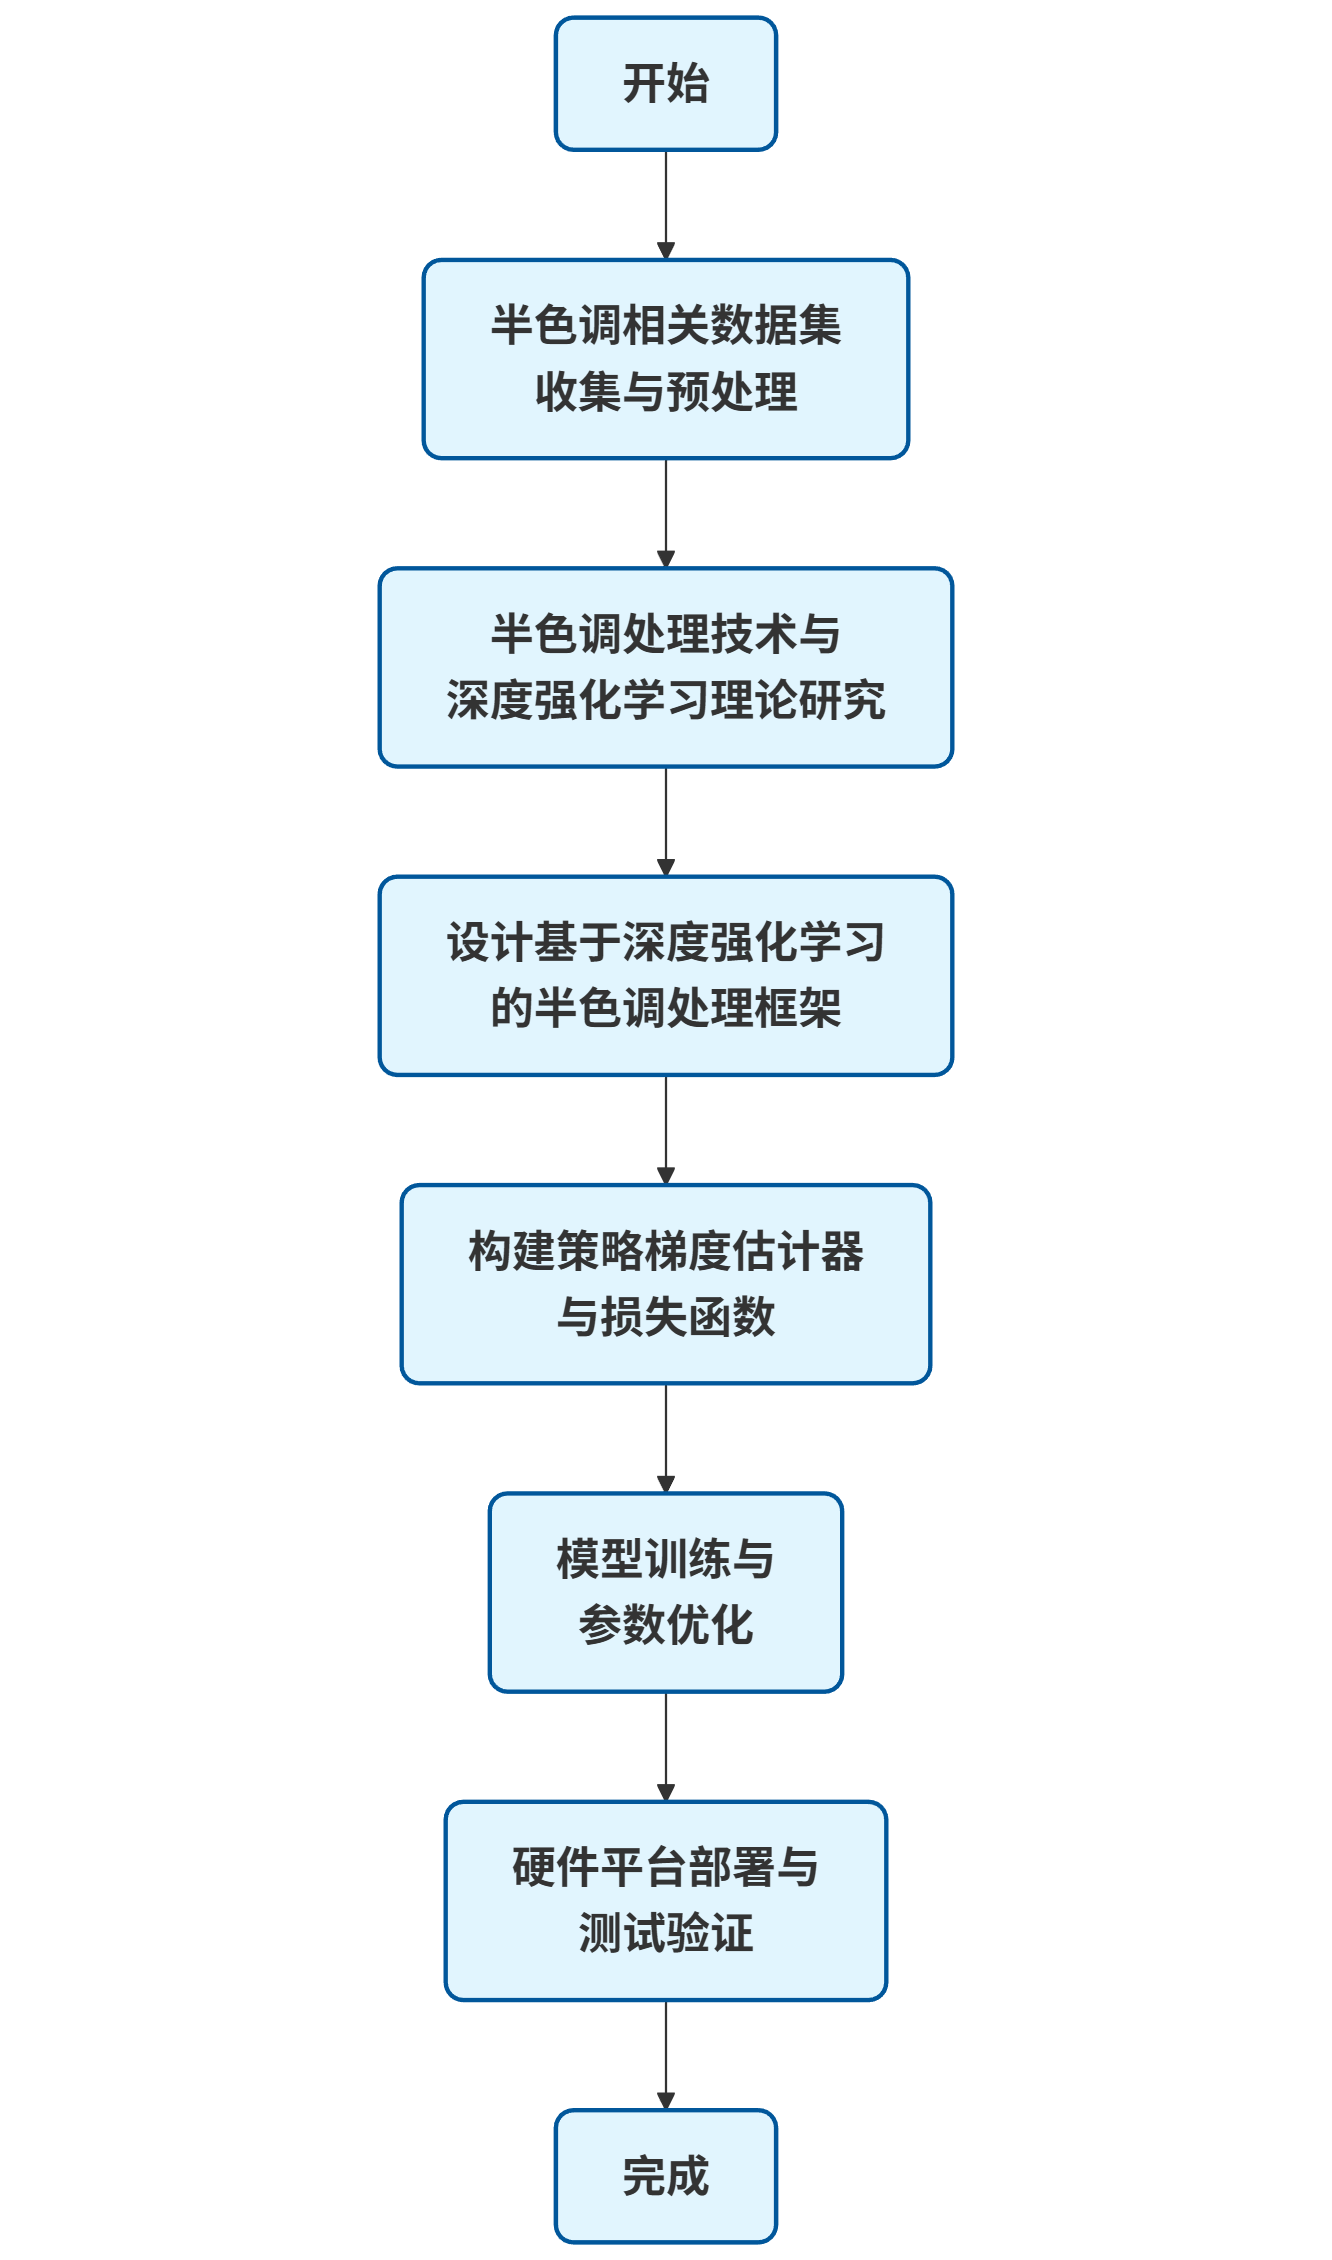
\includegraphics[width=0.58\textwidth]{../graphics/thesis/method/overall_workflow.png}
    \caption{基于强化学习的半色调生成总体流程}
    \label{fig:3-1}
\end{figure}

\subsection{状态、动作与单步多智能体建模}
在本文方法中，连续调图像 $c$ 提供稳定的亮度和结构上下文，高斯噪声图 $z$ 为策略在多解空间中提供随机性。策略网络输出概率图 $p=\pi_\theta(c,z)$，训练阶段对每个像素位置执行伯努利采样：
\begin{equation}
h_{ij}\sim\mathrm{Bernoulli}(p_{ij}),\qquad p_{ij}=\pi_\theta(c,z)_{ij}.
\label{eq:3-2}
\end{equation}
这样做的意义在于，同一连续调输入不再被绑定到唯一排列，而是允许策略在满足感知和频域约束的一族点阵中进行选择，这与蓝噪声本身具有随机排布属性的事实是一致的。

从多智能体视角看，每个像素都可以看作一个共享策略的虚拟智能体。虽然这些智能体没有独立网络副本，但共享参数的卷积结构保证了空间平移一致性和参数效率，同时又能通过感受野引入邻域上下文，使局部色调与纹理组织被统一纳入决策。由于任务只包含一次动作输出，没有长序列状态转移，因此本文采用的是单步多智能体强化学习而非多步交互式强化学习，这也使训练和部署过程更易落地。

\subsection{策略网络结构与设计依据}
本文采用的策略网络为一类轻量级全卷积残差网络。该模型以 2 通道输入开始，经过 1 层输入卷积、16 个残差块和 1 层输出卷积后，利用 Sigmoid 生成单通道概率图。每个残差块内部包含两层 $3\times3$ 卷积和 ReLU 激活，基础通道数设置为 32，卷积填充模式为 reflect。按卷积层数量统计，网络总计包含 33 层卷积；按当前参数配置估算，模型参数量约为 296833，属于典型的轻量级全卷积残差网络。

这一结构选择具有明确的任务针对性。首先，半色调属于对像素对齐极为敏感的底层视觉任务，若采用过多下采样和上采样操作，容易破坏局部统计与边缘定位，因此当前网络刻意保持原始分辨率不变，仅靠连续 $3\times3$ 卷积扩大感受野。其次，33 层卷积在步长为 1 的前提下可形成约 $67\times67$ 的理论感受野，足以覆盖半色调纹理形成所需的中尺度邻域。再次，残差结构比普通深层卷积更适合学习“在原始亮度约束附近做局部二值决策修正”的映射，能够提升训练稳定性\cite{HE2016Deep}。

与常见的编码器--解码器结构相比，当前网络没有引入多尺度瓶颈和复杂跳连，而是追求更规整的卷积计算路径。这一取舍意味着模型表达能力不是无限扩张的，但换来了更小的部署开销和更稳定的空间对齐特性。对于本文所关注的灰度半色调任务而言，这种选择是合理的。图 \ref{fig:3-2} 给出了网络结构示意图。

\begin{figure}[H]
    \centering
    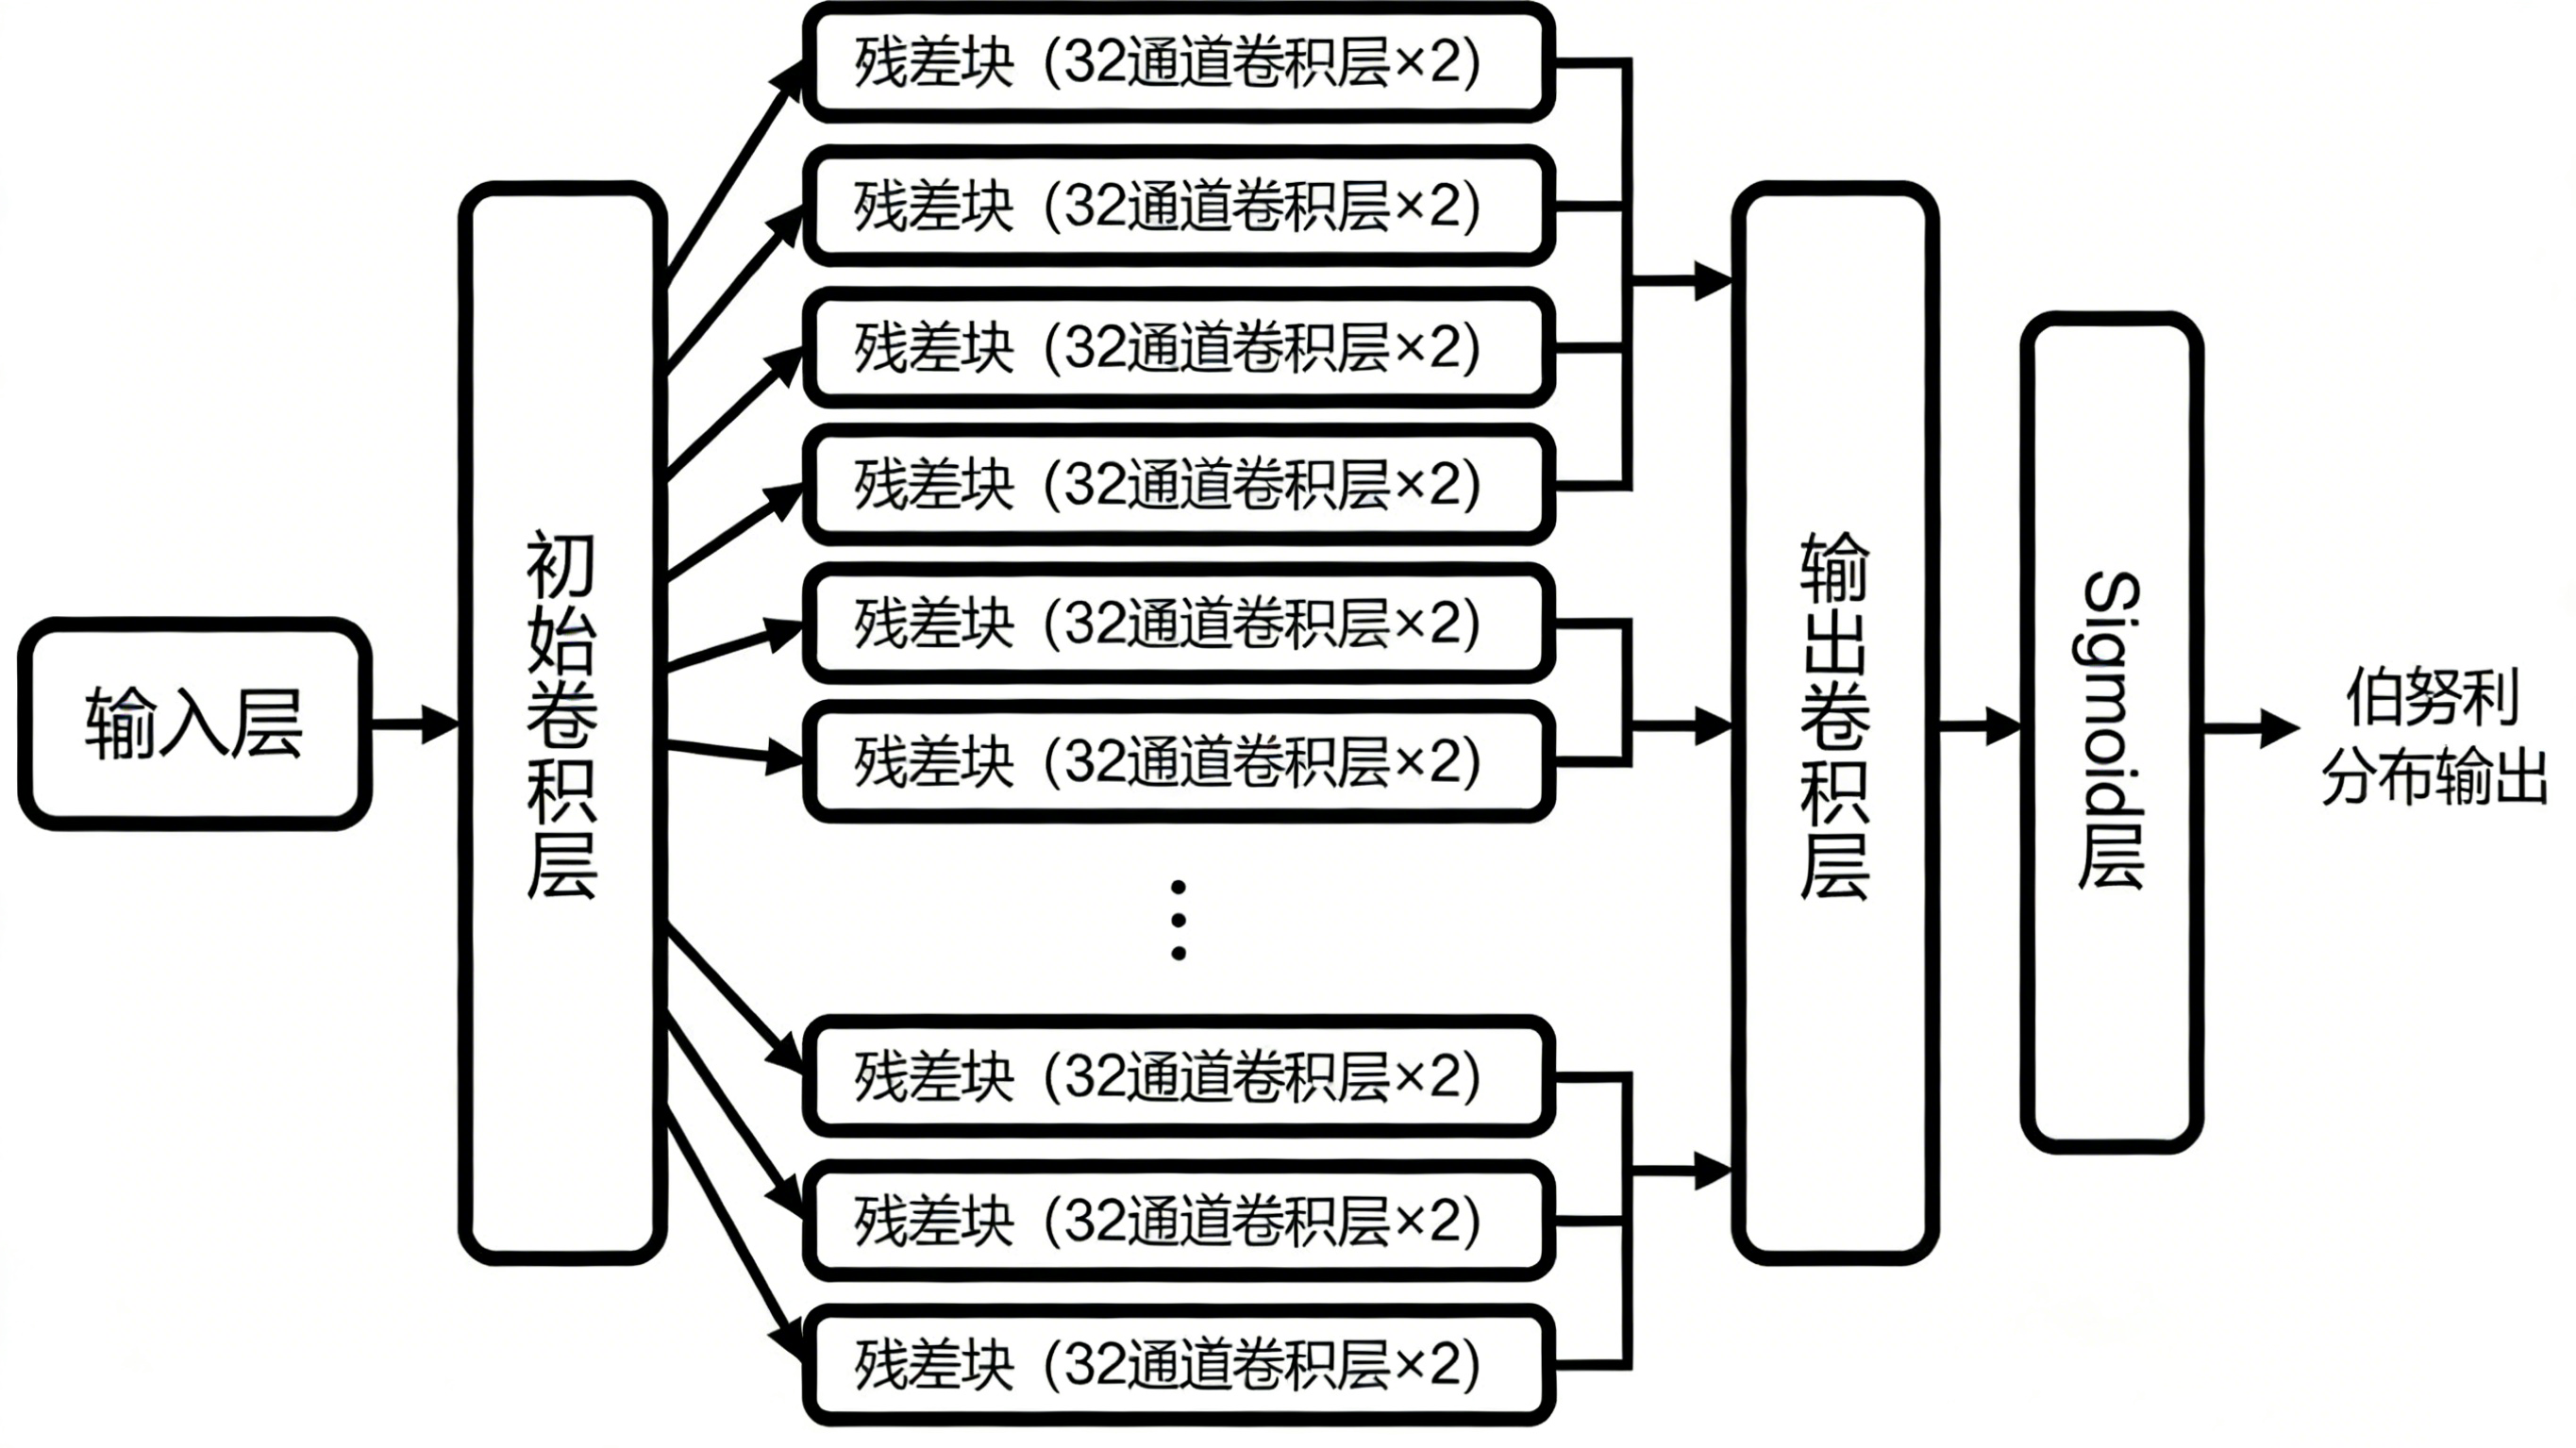
\includegraphics[width=0.96\textwidth]{../graphics/thesis/method/network_architecture.png}
    \caption{HalftoningPolicyNet 策略网络结构示意图}
    \label{fig:3-2}
\end{figure}

\subsection{奖励函数与辅助损失设计}
为了在离散动作空间中直接优化半色调质量，项目采用局部期望形式的多智能体强化学习损失。其核心思想不是把硬阈值强行松弛为普通可导函数，而是围绕离散动作的期望奖励进行近似优化。在奖励定义上，项目采用 HVS 误差与 CSSIM 的组合：
\begin{equation}
R(h,c)=-\left\|\operatorname{HVS}(h)-\operatorname{HVS}(c)\right\|_2^2+w_s\cdot\operatorname{CSSIM}(h,c),
\label{eq:3-3}
\end{equation}
其中结构项权重 $w_s$ 在当前配置中取 0.06。前一项强调观察尺度下的亮度一致性，后一项强调局部结构保持，两者共同约束“生成结果看起来是否仍像原图”。

仅依赖主奖励仍不足以保证概率图最终收敛到稳定二值端点。为进一步约束频域性质和阈值可部署性，项目在训练中加入了各向异性抑制项和高频混叠抑制项。总体训练目标可以表示为
\begin{equation}
L=L_{\mathrm{MARL}}+\lambda_{\mathrm{as}}L_{\mathrm{AS}}+\lambda_{\mathrm{alias}}L_{\mathrm{alias}},
\label{eq:3-4}
\end{equation}
其中当前配置下 $\lambda_{\mathrm{as}}=0.002$，$\lambda_{\mathrm{alias}}=0.002$。这表明项目并不希望辅助损失压倒强化学习主目标，而是将它们作为蓝噪声纹理的温和正则项。

从训练机制看，这一设计实际上包含三个层次。第一层是主奖励，负责把策略导向更好的感知质量；第二层是辅助频域损失，负责缓解方向性纹理和异常高频峰值；第三层是常灰度验收，负责检验最终概率输出是否真的可以安全阈值化。正是因为三者共同存在，本文方法才不至于停留在“采样结果看起来还不错”的表面成功上。

\subsection{训练验收闭环与工程约束}
根据配置文件，训练阶段使用 HalftoneVOC2012 训练集上的 $64\times64$ 随机裁块，训练批大小为 128，优化器采用 Adam，初始学习率设为 $3\times10^{-4}$，并通过 CosineAnnealingLR 逐步衰减到 $1\times10^{-5}$。模型主干采用 2 通道输入、32 个基础通道和 16 个残差块，输出端使用 Sigmoid 生成逐像素概率图。训练总轮数配置为 1000，最大迭代步数为 100000，这说明当前实现更强调在有限网络规模下获得稳定收敛。

训练验收的关键并不在于某一条损失曲线是否下降，而在于模型是否真正学会了“可阈值化的二值策略”。为此，项目在训练阶段引入了常灰度 suite，主验收灰度档位为 $\{0.2,0.4,0.5,0.6,0.8\}$，默认图像尺寸为 $256\times256$，批大小为 8。只有当 checkpoint 的常灰度端点聚集率达到 0.95 以上时，当前权重才会被接受为可靠候选模型。这样的验收口径使训练过程始终围绕可阈值化部署这一目标展开。

这种“主目标训练 + 常灰度强验收”的组织方式直接回应了半色调的部署需求。它使模型验收不再仅依赖自然图像上的平均指标，而是显式检查中灰区域是否已经形成稳定的双峰概率分布。对半色调任务而言，这一闭环比单纯降低训练损失更具决定性意义。

为了更清楚地概括训练、验收与部署之间的闭环关系，算法 \ref{alg:3-1} 改用与参考图相近的 procedure 伪代码风格，对离线训练阶段的随机裁块采样、联合损失优化，以及在线阶段的阈值化推理进行紧凑表达。与传统串行扫描式半色调不同，该流程把大部分复杂优化集中在离线训练阶段完成，从而为在线阶段保留了更规整、更易并行的前向推理路径。

\begin{algorithm}[H]
    \caption{基于强化学习的半色调训练与推理流程}
    \label{alg:3-1}
    \small
    \begin{algorithmic}
        \Procedure{训练}{$\mathcal{D}$}
            \State 初始化 $\theta$
            \Repeat
                \State 采样 $c\sim\mathcal{D},\ z\sim\mathcal{N}(0,\mathbf{I})$
                \State $p_\theta\gets\pi_\theta(c,z),\ h\sim\mathrm{Bernoulli}(p_\theta)$
                \State $\mathcal{L}_{\mathrm{joint}}\gets\mathcal{L}_{\mathrm{MARL}}+\lambda_{\mathrm{as}}\mathcal{L}_{\mathrm{AS}}+\lambda_{\mathrm{alias}}\mathcal{L}_{\mathrm{alias}}$
                \State $\theta\gets\theta-\alpha\nabla_{\theta}\mathcal{L}_{\mathrm{joint}}$
                \State $h_{\mathrm{thr}}\gets\mathbb{I}[p_\theta\ge 0.5]$
                \State $\rho_{\mathrm{end}}\gets\operatorname{EndpointRatio}(p_\theta;\mathcal{G})$
                \State $e_{\mathrm{tone}}\gets\operatorname{ToneError}(h_{\mathrm{thr}};\mathcal{G})$
            \Until{收敛且 $\rho_{\mathrm{end}}\ge 0.95$ 且 $e_{\mathrm{tone}}$ 稳定}
            \State \Return $\theta$
        \EndProcedure
        \Statex
        \Procedure{推理}{$c,\theta$}
            \State 采样 $z\sim\mathcal{N}(0,\mathbf{I})$
            \State $p_\theta\gets\pi_\theta(c,z)$
            \State $h\gets\mathbb{I}[p_\theta\ge 0.5]$
            \State \Return $h$
        \EndProcedure
    \end{algorithmic}
\end{algorithm}

\subsection{推理流程与边界处理}
推理阶段采用单次前向传播输出概率图，再通过 0.5 阈值得到二值半色调图像。为了减轻深层卷积网络在边界处感受野不完整的问题，本文的整图推理流程实现了自动感受野估计、边界镜像扩展与结果回裁。对于当前由 33 层 $3\times3$ 卷积组成的网络，可估算得到约 33 像素的感受野半径，因此在整图推理时需要在输入四周补充对应 halo，再在输出端裁回原始尺寸。

这一机制的价值在于，它不需要修改网络结构，也不依赖多尺度拼接策略，就能有效缓解边缘区域纹理不连续和感知指标偏移的问题。除输出最终半色调图像外，推理流程还会同步导出概率图、局部对比度权重图以及并排诊断图，为后续误差分析和论文插图提供直接素材。

\subsection{时间复杂度与部署成本分析}
在忽略常数项和 I/O 开销的情况下，当前网络的主要计算量由卷积层贡献。若用卷积层数 $L$、卷积核尺寸 $k$、通道数 $C$ 和图像尺寸 $H\times W$ 近似表示，其推理复杂度可写为
\begin{equation}
\mathcal{O}(Lk^2C^2HW).
\label{eq:3-5}
\end{equation}
由于网络没有显式注意力模块、多尺度金字塔或大型解码器，其计算路径相对规整，在线阶段可以保持一次前向传播的实现形式。

从部署接口看，当前模型输入为单通道连续调图像与单通道噪声图，输出为单通道概率图或阈值后的二值图，因此非常适合被封装成独立的半色调生成模块。需要指出的是，本文能直接验证的是 CUDA 环境下的推理潜力，而非所有硬件平台上的最终部署表现。CPU-only 延迟、量化后精度、不同设备点增益补偿等问题仍需后续补充实验。

\subsection{本章小结}
本章从建模、网络、损失、验收与推理五个层面系统说明了本文方法的设计逻辑。可以看到，强化学习并不是被简单作为一个流行标签附加到网络上，而是直接承担了离散动作建模的职责；常灰度验收也不是附带可视化，而是决定模型能否从训练阶段顺利过渡到部署阶段的关键机制。下一章将在这一方法基础上转入系统实现、训练配置和实验流程说明。

\section{系统实现、训练流程与关键工程细节}

\subsection{系统实现概览}
为了使论文章节与系统功能形成清晰映射，本文将 Halftoning 系统划分为模型定义、损失计算、训练调度、整图推理、实验验证和结果归档六个层次。与许多只强调最终网络结构的论文不同，本文特别强调工程链路的完整性，因为半色调任务的结论可信度不仅取决于模型本身，也取决于训练如何验收、结果如何归档以及指标如何复核。

表 \ref{tab:4-1} 给出了核心功能模块与论文内容之间的对应关系。可以看到，每个关键论述都能在系统实现层面找到对应落点：训练主流程负责参数更新与候选模型保存，整图推理流程负责边界处理与结果导出，离线评测流程负责实验统计与结果汇总，感知损失与评价统计模块则共同支撑方法设计与实验分析。

\begin{table}[H]
    \centering
    \small
    \caption{系统主要功能模块与职责映射}
    \label{tab:4-1}
    \begin{tabularx}{0.98\textwidth}{>{\raggedright\arraybackslash}p{0.20\textwidth}YY}
        \toprule
        模块类别 & 主要职责 & 与论文内容的对应关系 \\
        \midrule
        训练主流程模块 & 参数更新、优化器与调度器维护、候选模型保存 & 训练策略、验收闭环、日志记录 \\
        整图推理模块 & 整图推理、halo padding、结果导出与运行时统计 & 推理流程、边界处理、案例分析 \\
        离线评测模块 & 候选测试集复核、常灰度频谱分析、运行时测量 & 主实验结果、常灰度结果、效率分析 \\
        策略网络定义模块 & 策略网络结构定义与前向传播 & 网络结构与参数规模 \\
        感知损失模块 & HVS、CSSIM、MARL 主损失及辅助项计算 & 奖励函数与联合优化目标 \\
        指标统计模块 & 感知指标、蓝噪声指标、端点聚集率计算 & 评价体系与实验统计 \\
        结果归档模块 & 主结果、目标探针与运行时数据归档 & 表格来源与证据链组织 \\
        \bottomrule
    \end{tabularx}
\end{table}

\subsection{数据组织与实验划分}
    根据实验配置，系统将数据划分为训练集、验证集和小规模测试集三部分。此外，整图复核阶段还从未参与训练与验证的自然图像中构建了一个包含 1684 张图像的候选测试集，用于更加稳定地评估整图指标。该拆分口径与主结果归档统计保持一致，能够为论文中的主结果表提供直接依据。

从实验组织角度看，这一划分具有两个特点。其一，训练和验证阶段可以采用裁块形式提升吞吐，而论文汇报阶段则使用整图评价口径，避免裁块边界对感知指标的影响。其二，项目同时保留了自然图像测试与常灰度合成测试两条验证线：前者回答“模型在真实图像上的总体效果如何”，后者回答“模型是否真正形成了可部署的二值蓝噪声策略”。这种双线验证结构正是本文实验章节的组织基础。

\subsection{实验环境与关键配置}
除归档主结果外，本文在补充传统基线复评、频谱可视化和论文图表生成阶段，也使用当前实验平台完成了附加验证。当前本地平台采用 AMD Ryzen 7 9700X 8-Core Processor 和 NVIDIA GeForce RTX 5080，软件环境为 Windows 10、Python 3.10.11、PyTorch 2.10.0+cu128 与 CUDA 12.8。

对本科论文而言，更重要的是把“运行平台”和“直接影响实验结果的训练配置”区分开来：前者用于说明补充复评和图表生成所处的硬件软件条件，后者则用于交代模型训练、验证和验收所依赖的关键设置。当前补充复评与图表生成工作在 Windows 10 22H2 环境下完成，硬件平台为 AMD Ryzen 7 9700X 8-Core Processor 与 NVIDIA GeForce RTX 5080，软件环境为 Python 3.10.11、PyTorch 2.10.0+cu128、CUDA Runtime 12.8 与 cuDNN 9.10。

项目核心训练与验证配置改用文字描述如下：模型以连续调图像和噪声图组成的 2 通道输入为基础，主干设置 32 个基础通道与 16 个残差块，输出端使用 Sigmoid 生成逐像素概率图。训练阶段采用 $64\times64$ 随机裁块，训练与常规验证的批大小均为 128；优化器为 Adam，初始学习率设为 $3\times10^{-4}$，并通过 CosineAnnealingLR 逐步衰减至 $1\times10^{-5}$。训练总轮数配置为 1000，最大迭代步数为 100000。

在目标设计上，主奖励结构项权重 $w_s$ 设为 0.06，各向异性损失权重与混叠抑制损失权重均设为 0.002。训练过程的主验收依赖常灰度 suite，灰度档位取 $\{0.2,0.4,0.5,0.6,0.8\}$，评价图像尺寸为 $256\times256$、批大小为 8；只有当候选 checkpoint 的端点聚集率达到 0.95 以上时，当前权重才被视为通过验收。这些设置共同体现了本文更关注“训练后能否稳定阈值化部署”，而不仅是损失曲线是否下降。

\subsection{训练、验证与推理流程}
训练流程由训练脚本驱动，大致可以分为四个阶段，图 \ref{fig:4-1} 对其核心闭环进行了概括。第一阶段是数据准备与随机裁块，从训练集中采样 $64\times64$ 连续调块输入策略网络。第二阶段是策略采样与联合损失计算，网络输出概率图后，对应计算 MARL 主损失、CSSIM 奖励和频域辅助损失。第三阶段是周期性验证，记录自然图像指标与常灰度 suite 指标，并根据端点聚集率决定是否接受当前 checkpoint。第四阶段是训练日志和缓存结果保存，为后续复核保留结构化记录。

\begin{figure}[H]
    \centering
    \resizebox{0.96\textwidth}{!}{%
    \begin{tikzpicture}[
        node distance=8mm and 8mm,
        process/.style={rectangle, rounded corners=2pt, draw=black, fill=gray!10, minimum width=30mm, minimum height=8mm, align=center},
        decision/.style={diamond, draw=black, fill=gray!5, aspect=2.2, inner sep=1.5pt, align=center},
        arrow/.style={-{Latex[length=2mm]}, thick}
    ]
        \node[process] (data) {训练集样本\\随机裁块与噪声生成};
        \node[process, right=of data] (forward) {策略网络前向\\输出概率图};
        \node[process, right=of forward] (loss) {MARL 主目标\\CSSIM 与频域辅助项};
        \node[process, right=of loss] (update) {反向传播\\更新参数};

        \node[process, below=14mm of forward] (validate) {自然图像验证\\常灰度 suite 评估};
        \node[decision, right=16mm of validate] (accept) {端点聚集率与\\色调误差达标?};
        \node[process, right=16mm of accept] (save) {保存候选\\checkpoint};
        \node[process, left=16mm of accept] (continue) {继续训练\\进入下一轮验证};

        \draw[arrow] (data) -- (forward);
        \draw[arrow] (forward) -- (loss);
        \draw[arrow] (loss) -- (update);
        \draw[arrow] (update) |- (validate);
        \draw[arrow] (validate) -- (accept);
        \draw[arrow] (accept) -- node[above,font=\small]{是} (save);
        \draw[arrow] (accept) -- node[above,font=\small]{否} (continue);
        \draw[arrow] (save.south) |- ++(0,-8mm) -| (data.south);
        \draw[arrow] (continue.south) |- ++(0,-8mm) -| (data.south);
    \end{tikzpicture}
    }
    \caption{训练、验证与 checkpoint 验收流程图}
    \label{fig:4-1}
\end{figure}

该流程图突出了本文与普通图像到图像回归训练的一个区别，即 checkpoint 是否被接受并不只依赖自然图像上的平均指标，而是必须结合常灰度输入下的端点聚集率与阈值色调误差共同判断。这一设计使训练过程从一开始就与最终部署目标保持对齐。

推理流程由整图推理模块完成。该流程首先加载训练好的策略网络，自动估计感受野半径，再对输入图像实施 halo padding。前向传播结束后，系统会导出最终半色调图、概率图、局部对比度权重图以及并排诊断图。其中概率图用于分析模型是否已经端点收敛，局部对比度权重图用于观察 CSSIM 的空间权重分布，并排诊断图则把输入、对比度图、概率图与阈值结果放在一起，便于论文中的定性案例分析。

验证和结果整理主要由离线评测与汇总流程完成。该流程提供候选测试集整图统计、小规模测试样本统计、常灰度频谱可视化和 512\(\times\)512 运行时测量等功能。换言之，论文中使用的大多数表格和关键图像，并不是人工手工整理得到，而是由统一评测流程自动生成并归档。这种组织方式显著降低了转录误差和口径漂移的风险。

\subsection{结果归档与证据链组织}
为了使实验结论可追溯，本文将不同用途的结果分别保存为结构化归档结果。主统计归档结果负责记录候选测试集、小规模测试样本和常灰度验收集的主统计量，是论文主结果表和常灰度表的直接来源；机制探针归档结果负责记录 baseline、最终模型以及局部梯度探针结果，用于解释“为什么仅凭采样结果并不能保证阈值部署正确”；运行时归档结果则记录运行时统计参数与平均耗时，是效率分析的依据。

从论文写作角度看，这种归档方式的价值在于，它把“现象”“原因”和“部署意义”拆分为不同层级的证据。自然图像均值用于回答总体效果，常灰度验收结果用于回答端点收敛和蓝噪声行为，目标探针用于回答机制解释，运行时统计用于回答工程潜力。通过把这些证据沿着相同的问题链条组织起来，论文就能避免只堆砌图表而缺乏论证逻辑的问题。

\subsection{实验复现流程与关键日志解读}
为了让第 4 章真正承担“系统实现可复核”的作用，本文不把复现实验理解为笼统的“重新运行代码”，而是把它拆分为训练、整图推理、统一复评和论文图表整理四个可追踪环节。其最小复现单元由统一配置、候选权重、结构化统计结果和图像归档资源共同组成：训练环节负责完成参数更新与候选权重验收，整图推理环节负责导出诊断图与二值结果，离线复评环节负责汇总主结果、常灰度分析与运行时统计，图表整理环节则把结构化结果转写为论文中的插图资源。

表 \ref{tab:4-3} 将这些关键环节的输入、输出和论文用途对应起来。这样做的价值在于，当评审追问“某张图或某个数字具体来自哪里”时，论文能够直接回到相应流程与归档结果，而不是依赖人工回忆实验过程。这种“流程环节-归档结果-论文图表”三段式映射，也是本章强调工程证据链的核心原因。

\begin{table}[H]
    \centering
    \small
    \caption{实验复现链路中的关键环节、输入输出与论文用途}
    \label{tab:4-3}
    \begin{tabularx}{0.98\textwidth}{>{\raggedright\arraybackslash}p{0.16\textwidth}>{\raggedright\arraybackslash}p{0.24\textwidth}YY}
        \toprule
        流程环节 & 主要输入 & 主要输出 & 在论文中的作用 \\
        \midrule
        训练与候选验收流程 & 统一配置、训练/验证数据与已有候选权重 & 候选模型权重、训练缓存序列与阶段性验收记录 & 支撑训练收敛、候选权重筛选、常灰度门控与训练稳定性讨论 \\
        整图推理流程 & 候选权重、待测图像与推理配置 & 半色调结果、概率诊断图、局部对比度图和整图评价摘要 & 支撑整图推理流程、边界处理说明、定性案例和诊断图来源 \\
        离线统一复评流程 & 候选权重、常灰度验收集、候选测试集与运行时测量设置 & 主结果统计、运行时统计、常灰度频谱图与训练稳定性图 & 支撑主结果表、常灰度分析、运行时统计和训练稳定性图 \\
        论文图表整理流程 & 已归档的统计结果、基线结果与示例图像 & 论文中的比较图、频谱图和诊断插图 & 将结构化实验结果转写为论文插图，减少手工转录误差 \\
        \bottomrule
    \end{tabularx}
\end{table}

    从日志解读角度看，训练阶段最值得关注的不是某一次 batch 的瞬时波动，而是训练缓存中的总损失、主损失、频域辅助损失以及相应梯度范数序列，是否与常灰度验收结果同步进入稳定区间。离线复评流程会将这些缓存序列整理为训练稳定性图，并同步生成主结果统计、运行时统计和常灰度频谱可视化，使“训练是否收敛”“阈值部署是否稳定”“整图运行是否足够快”三个问题分别对应到不同证据载体。

    若按较稳妥的实验复现顺序执行，应先进行训练或基于已有候选权重恢复训练，检查训练阶段的奖励、损失和常灰度验收统计，确认模型已经进入稳定收敛区间；其次在少量代表性整图样本上做快速一致性检查，排除明显色调漂移或边界异常；再次在候选测试图像和常灰度验收集上完成统一口径统计；最后再整理论文插图。这样的顺序既能降低大规模复评成本，也避免在模型尚未通过常灰度验收时过早投入整图统计和图表整理。

    训练日志的阶段性变化本身也值得被写入论文。一般而言，训练早期的主要任务是建立基本的亮度映射能力，此时 MARL 主损失波动较大但很快靠近 0；中期阶段辅助频域项逐步参与，使常灰度样本的各向异性和混叠能量进入更稳定区间；后期阶段若设置合理，概率标准差和端点聚集率会迅速上升，说明模型开始真正具备可阈值化的二值输出能力。把这一过程与训练缓存中的序列统计以及常灰度结果结合起来解读，有助于说明本文不是简单展示一条损失曲线，而是在解释模型从“可采样”走向“可部署”的全过程。

    此外，关键配置、候选权重和结构化结果共同构成了实验的最小复现闭环。训练、推理与复评流程都显式依赖统一配置，整图推理还要求给定模型权重与输出位置；主结果统计、运行时统计和案例图像再沉淀为结构化记录与图像资源。这使得论文中的关键数值不仅来自实验输出，还能够回溯到具体流程、具体配置和具体归档结果，进而为后续补做基线实验或重新训练提供统一起点。

\subsection{本章小结}
本章从系统模块、数据划分、关键配置、训练流程和结果归档五个方面说明了当前实现如何支撑本文的研究与写作。与只关注模型结构的描述方式相比，本文更强调训练验收、结果归档和实验复核的完整性，因为这些环节共同决定了后续实验结论是否可信。下一章将在此基础上对主结果、常灰度行为、目标探针和案例图像进行综合分析。

\section{实验设计、结果分析与基线比较}

\subsection{实验目标与评价协议}
本章实验围绕四个问题展开：第一，模型在自然图像整图评价口径下能达到怎样的总体质量；第二，模型在常灰度输入下是否已经形成稳定的蓝噪声纹理和端点收敛；第三，训练目标为何能够或不能够自然推动概率图走向可部署的二值状态；第四，该方法与传统半色调路线相比处在怎样的研究定位上。为回答这些问题，本文同时使用 CSSIM、SSIM、Gaussian-HVS PSNR、Nasanen-HVS PSNR、各向异性值、混叠能量和端点聚集率等指标。

需要说明的是，本章中的强化学习主结果主要来自项目已经保存并核对过的验证文件，而不是本次写作过程中重新完整训练得到；与此同时，本文又在相同评价协议下补充重跑了传统基线实验。也正因如此，论文在论述中会明确区分“已归档并核对过的主模型结果”“本次统一复评得到的基线结果”和“代码中可直接验证的实现逻辑”。这种口径处理虽然更克制，但也更符合本科毕业论文对真实性和可核验性的要求。

\subsection{候选测试集主结果分析}
表 \ref{tab:5-1} 汇总了 1684 张候选测试图像上的主要指标，并同时给出既有归档统计中的论文目标均值。可以看到，当前模型在 CSSIM 和 Gaussian-HVS PSNR 上已经非常接近目标均值，SSIM 略高于目标均值；相比之下，Nasanen-HVS PSNR 仍有约 1.25 dB 的差距，说明在更严格的人眼低通观察模型下，模型仍存在可提升空间。

\begin{table}[H]
    \centering
    \caption{1684 张候选测试图像上的主要结果}
    \label{tab:5-1}
    \begin{tabular}{lccc}
        \toprule
        指标 & 当前结果 & 目标均值 & 差值 \\
        \midrule
        CSSIM & 0.9226 & 0.9236 & -0.0010 \\
        SSIM & 0.1637 & 0.1610 & +0.0027 \\
        Gaussian-HVS PSNR / dB & 37.4555 & 37.5470 & -0.0915 \\
        Nasanen-HVS PSNR / dB & 30.3879 & 31.6420 & -1.2541 \\
        各向异性 / dB & 0.0953 & -- & -- \\
        \bottomrule
    \end{tabular}
\end{table}

除表中指标外，候选测试集上的 reward 均值为 0.0544。这意味着在 HVS 误差与 CSSIM 奖励共同作用下，策略网络已经形成一套稳定的局部二值生成规则。若结合 4 张小规模整图验证样本的结果继续观察，还可以看到 CSSIM 达到 0.9521，Gaussian-HVS PSNR 达到 37.80 dB，Nasanen-HVS PSNR 达到 30.52 dB，整体上略高于大规模候选集的均值。这一现象说明当前模型对主体清晰、对比度较强的图像更容易取得较好表现，而在复杂纹理、低对比背景或弱边缘过渡场景中，仍会拉低整体感知指标。

从结果解释上看，CSSIM 与 Gaussian-HVS PSNR 已接近目标均值，说明模型在主体结构保持和较平滑观察尺度下的亮度还原方面已经具备较强能力；而 Nasanen-HVS PSNR 的差距提示我们，针对更严格视觉建模的误差控制仍是后续优化重点。这种“不同指标成熟度不完全一致”的现象并不意味着方法失效，而是为后续实验改进指明了更具体的方向。

\subsection{统一口径下的传统基线对比}
为避免不同数据划分、观察模型和实现细节带来的比较偏差，本文在与主实验一致的数据划分和评价协议下，对 Bayer 8\(\times\)8 有序抖动\cite{BAYER1973An} 和 Floyd-Steinberg 误差扩散\cite{FLOYD1976An} 进行了统一复评。复评过程使用与主实验一致的 CSSIM、SSIM、两类 HVS-PSNR 与各向异性统计口径，因此得到的基线结果可用于与本文强化学习模型进行更直接的横向比较。

\begin{table}[H]
    \centering
    \small
    \caption{统一评价协议下传统基线与强化学习方法的候选测试集对比}
    \label{tab:5-1b}
    \setlength{\tabcolsep}{4pt}
    \begin{tabular}{lccccc}
        \toprule
        方法 & CSSIM & SSIM & \shortstack{Gaussian-HVS\\PSNR / dB} & \shortstack{Nasanen-HVS\\PSNR / dB} & \shortstack{各向异性\\/ dB} \\
        \midrule
        强化学习方法 & 0.9226 & 0.1637 & 37.4555 & 30.3879 & 0.0953 \\
        Bayer 有序抖动 & 0.9062 & 0.0726 & 34.3460 & 29.5877 & -6.7828 \\
        Floyd-Steinberg 误差扩散 & 0.9119 & 0.1090 & 40.1235 & 31.1984 & -0.2207 \\
        \bottomrule
    \end{tabular}
\end{table}

图 \ref{fig:5-1b} 将表 \ref{tab:5-1b} 中最核心的四项指标进行了可视化。与仅通过表格逐列阅读相比，柱状图更直观地显示出三条路线的差异分工：本文方法在 CSSIM 和 SSIM 上占优，说明其在主体结构与局部对比保持方面更具优势；Floyd-Steinberg 在两类 HVS-PSNR 上更强，说明其局部亮度守恒机制在观察尺度重建方面仍然非常有效；Bayer 有序抖动则在四项指标上整体落后，体现出模板化方法在复杂自然图像上的局限。

\begin{figure}[H]
    \centering
    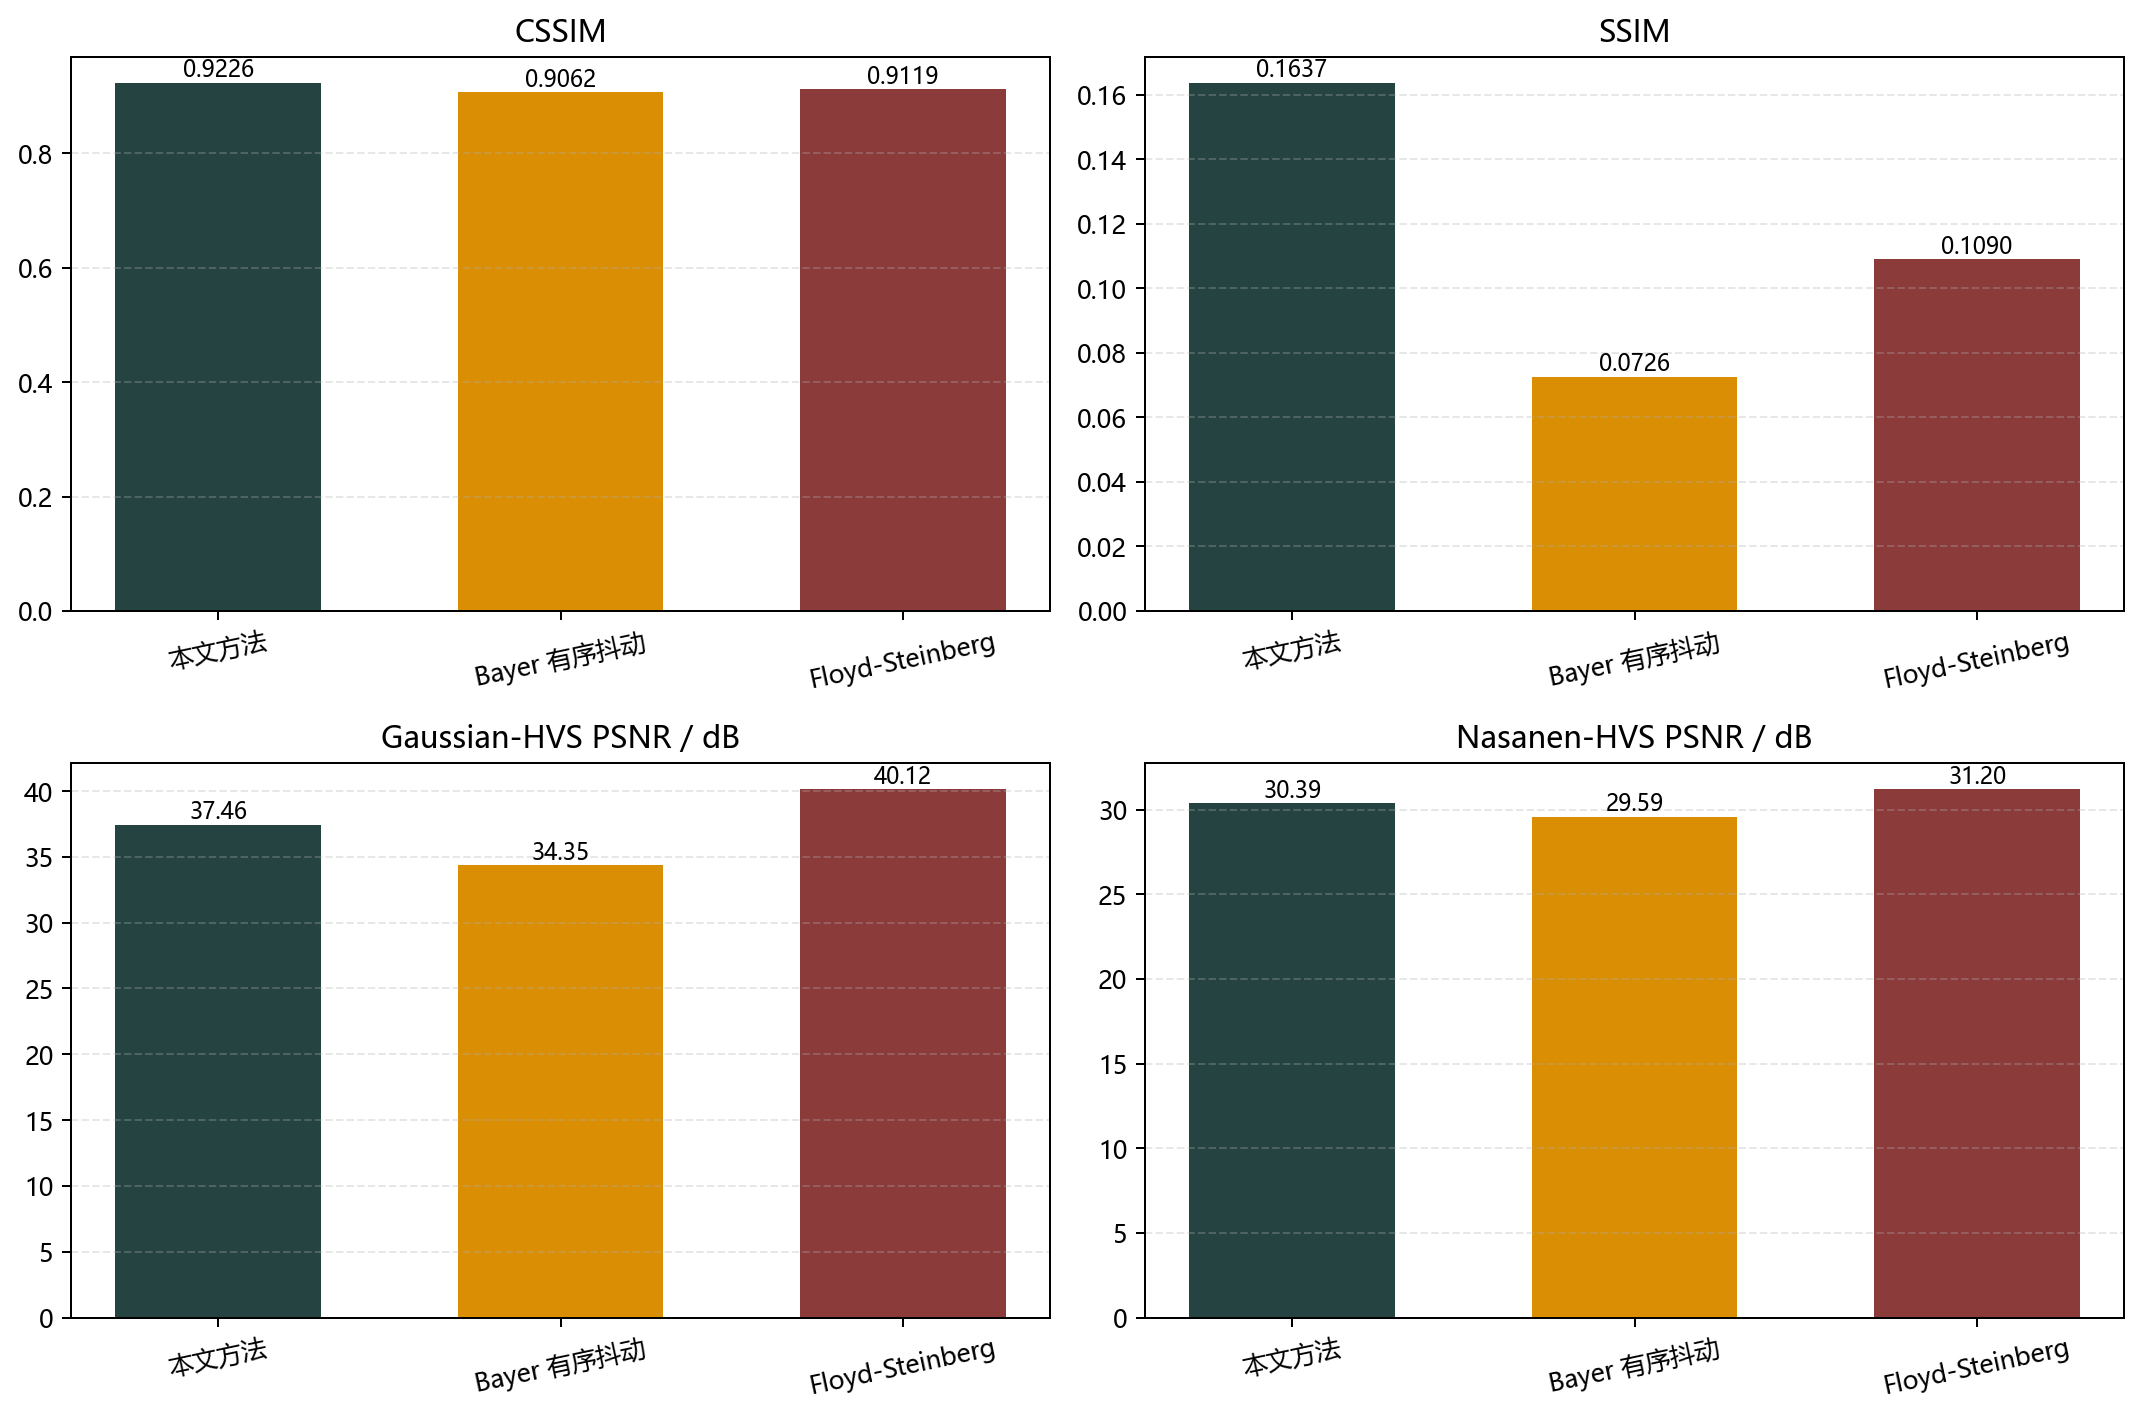
\includegraphics[width=0.96\textwidth]{../graphics/thesis/5-7_candidate_metric_comparison.png}
    \caption{候选测试集上三类方法的主要指标可视化对比}
    \label{fig:5-1b}
\end{figure}

从候选测试集均值可以看到，Bayer 有序抖动在各项自然图像指标上均明显落后：其 CSSIM 为 0.9062，Gaussian-HVS PSNR 为 34.3460 dB，Nasanen-HVS PSNR 为 29.5877 dB，说明固定阈值模板虽然实现简单，但在当前数据划分和观察模型下难以兼顾结构保持与感知质量。相比之下，Floyd-Steinberg 误差扩散仍然是一个非常强的传统基线，其 Gaussian-HVS PSNR 和 Nasanen-HVS PSNR 分别达到 40.1235 dB 和 31.1984 dB，均高于本文方法。

如果把这些差异放回方法机制中理解，Floyd-Steinberg 在两类 HVS-PSNR 上领先并不意外。该算法通过逐像素传播量化误差，显式维持局部平均亮度守恒，因此在人眼低通观察模型下更容易获得较高的亮度重建分数；但这种优势是以串行扫描和路径依赖为代价换来的。本文方法虽然在观察尺度亮度误差上仍落后于误差扩散，但策略网络能够结合更大感受野和 CSSIM 奖励，对主体轮廓、边缘对比和局部结构连续性施加更直接的优化压力，因此在 CSSIM 和 SSIM 上仍保持优势。这说明当前强化学习方法真正优化的并不是单一亮度误差，而是“亮度、结构和部署一致性”的综合目标。

但这并不意味着强化学习方法失去研究价值。首先，从结构相关指标看，本文方法的 CSSIM 为 0.9226，高于 Floyd-Steinberg 的 0.9119，也明显高于 Bayer 有序抖动的 0.9062；SSIM 同样达到 0.1637，高于两类传统基线。其次，从项目内部组合奖励看，本文方法在候选测试集上的 reward 均值为 0.0544，仍略高于 Floyd-Steinberg 的 0.0539 和 Bayer 有序抖动的 0.0533，说明在 HVS 误差与结构奖励的联合口径下，强化学习方法仍能取得更均衡的综合表现。再次，从各向异性指标看，本文方法与 Floyd-Steinberg 都接近 0 dB，其中前者为 0.0953 dB，后者为 -0.2207 dB，二者都明显优于 Bayer 有序抖动的 -6.7828 dB。这表明当前方法并不是在所有指标上无条件压倒传统误差扩散，而是在保持一次前向并行推理、较好结构保真和稳定部署证据链的前提下，提供了不同于经典串行算法的折中方案。

有序抖动在各向异性指标上的明显劣势也具有直接的频域解释。固定 Bayer 阈值矩阵天然带有周期性方向结构，复制到整幅图像后会在频谱中形成更规则的能量峰，因此统一复评后其各向异性均值达到 -6.7828 dB，远离本文方法和 Floyd-Steinberg 附近的近零水平。换言之，Bayer 有序抖动的主要问题并不只是“分数偏低”，而是它更容易在规则纹理、平坦背景和重复结构中暴露出模板痕迹。对比之下，本文方法虽然不是所有指标上的最优者，但在自然图像结构保持、近零 dB 各向异性和并行推理方式之间取得了更符合现代图像预处理链路的综合平衡，这也是其在本科毕业论文中值得单独讨论的原因。

图 \ref{fig:5-1c} 给出了代表性机场场景图像上的视觉结果与傅里叶频谱对比。从空间域看，Bayer 有序抖动在天空、地面和机身过渡区域中保留了明显的规则网格痕迹；Floyd-Steinberg 误差扩散在亮度重建上更平滑，但仍然可见沿扫描方向延伸的弱结构条带；本文方法在机身文字、机翼轮廓和塔台边缘附近保留了更清晰的结构，同时其频谱中心附近的低频能量抑制更明显，外围高频能量分布也相对均匀。这一图像层面的现象与前文关于 CSSIM、各向异性和蓝噪声纹理的定量分析是一致的。

\begin{figure}[H]
    \centering
    \includegraphics[width=0.98\textwidth]{../graphics/thesis/5-6_fourier_spectrum_case_comparison.png}
    \caption{代表性图像上的半色调结果与傅里叶频谱对比}
    \label{fig:5-1c}
\end{figure}

这一结论在 4 张小规模整图验证样本上也呈现出相似趋势：本文方法的 CSSIM 为 0.9521，仍高于 Bayer 有序抖动的 0.9451 和 Floyd-Steinberg 的 0.9475；而 Floyd-Steinberg 在两类 HVS-PSNR 上依然占优。换言之，统一基线实验并没有把本文方法简单推向“全面领先”或“完全失效”的单一结论，而是更准确地揭示了不同技术路线在结构保持、观察尺度亮度误差、频谱均衡性和部署方式上的取舍差异。这种更克制的比较结果，也更符合本科毕业论文应有的真实性标准。

表 \ref{tab:5-1c} 进一步给出了 primary\_small\_split 上的统一对比结果。由于这 4 张图像主体更集中、边缘更清晰，强化学习方法在 CSSIM 和 reward 上的优势更容易被放大，而 Floyd-Steinberg 仍在两类 HVS-PSNR 上保持领先。这种“小样本更看结构、大样本更看总体稳定”的差异，与前文关于不同图像内容会拉开指标侧重点的分析是一致的。

\begin{table}[H]
    \centering
    \small
    \caption{primary\_small\_split 上统一基线实验的补充结果}
    \label{tab:5-1c}
    \setlength{\tabcolsep}{3pt}
    \begin{tabular}{lcccc}
        \toprule
        方法 & CSSIM & reward & \shortstack{Gaussian-HVS\\PSNR / dB} & \shortstack{Nasanen-HVS\\PSNR / dB} \\
        \midrule
        强化学习方法 & 0.9521 & 0.0562 & 37.8006 & 30.5190 \\
        Bayer 有序抖动 & 0.9451 & 0.0558 & 36.3613 & 30.3253 \\
        Floyd-Steinberg 误差扩散 & 0.9475 & 0.0561 & 41.2034 & 31.2096 \\
        \bottomrule
    \end{tabular}
\end{table}

若进一步比较候选测试集上的跨图像离散程度，还可以发现本文方法在 CSSIM 上的标准差为 0.0260，小于 Floyd-Steinberg 的 0.0335 和 Bayer 有序抖动的 0.0381。这说明强化学习策略虽然并未在每一张图像上都取得最高亮度重建分数，但在结构相似度这一更贴近本文任务目标的指标上，表现出更稳定的总体控制能力。换言之，统一基线实验的意义不只是给出一组“谁高谁低”的数字，而是帮助我们识别：误差扩散更擅长局部亮度守恒，强化学习方法更擅长在多类自然图像上维持结构质量和部署一致性的整体平衡。

\subsection{常灰度 suite 与蓝噪声行为分析}
自然图像均值能够说明模型总体是否可用，但难以直接回答概率图是否已经真正收敛到二值端点。为此，本文进一步分析常灰度验收集。根据主统计归档结果，整体端点聚集率达到 0.9957，中灰区域端点聚集率达到 0.9954，阈值色调误差仅为 0.0018，说明模型输出的概率图已经高度集中到 0 和 1 两端，并且经过固定阈值后几乎不会引入额外色调偏移。这一结论对部署尤其重要，因为实际系统更可能使用固定阈值而非继续随机采样。

表 \ref{tab:5-2} 选取训练主验收使用的 5 个灰度档位，展示其代表性统计结果。可以看到，0.2 至 0.8 各档位的端点聚集率均高于 0.994，阈值白像素比例与输入灰度高度一致；其中 0.5 灰度下的概率标准差达到 0.4993，说明中灰区域已经形成典型的双峰化分布，而不再停留在 0.5 附近的大量模糊中间状态。

\begin{table}[H]
    \centering
    \caption{常灰度主验收档位上的关键统计结果}
    \label{tab:5-2}
    \begin{tabular}{ccccc}
        \toprule
        输入灰度 & 端点聚集率 & 概率标准差 & 阈值白像素比例 & 阈值各向异性 / dB \\
        \midrule
        0.2 & 0.9963 & 0.3958 & 0.1959 & 0.4083 \\
        0.4 & 0.9946 & 0.4880 & 0.3972 & 0.0804 \\
        0.5 & 0.9969 & 0.4993 & 0.4989 & 0.0128 \\
        0.6 & 0.9946 & 0.4887 & 0.5999 & 0.0116 \\
        0.8 & 0.9956 & 0.3975 & 0.8016 & 0.2350 \\
        \bottomrule
    \end{tabular}
\end{table}

图 \ref{fig:5-1} 给出了常灰度输入下的概率图、采样图、频谱图和阈值图。从图中可以直观看到，随着输入灰度从 0.2 提升到 0.8，黑白点密度平滑变化，阈值图与采样图在整体统计上保持一致；尤其在 0.4 至 0.6 的中灰区间，频谱中心附近形成了较明显的低频抑制区域，外围能量分布相对均匀，符合蓝噪声“压低低频、扩散高频”的典型特征。这说明本文方法不仅在统计指标上达到高端点聚集率，也在可视化层面呈现出较自然的半色调纹理。

\begin{figure}[H]
    \centering
    \includegraphics[width=0.98\textwidth]{../graphics/thesis/constant_gray_spectrum.png}
    \caption{常灰度输入下的概率图、采样结果、频谱图与阈值结果}
    \label{fig:5-1}
\end{figure}

值得注意的是，训练阶段的主验收仅使用 5 个灰度档位，而离线复核阶段还补充评估了 0.1 到 0.9 的九档常灰度输入。这种做法使训练时的监控成本和论文阶段的分析深度得以兼顾，也说明当前实验体系并非只在个别灰度上偶然有效，而是在整个灰度区间内都具备较稳定的端点与纹理表现。

\subsection{训练稳定性与运行效率}
图 \ref{fig:5-2} 展示了训练过程中 total\_loss、marl\_loss 和 las\_loss 的局部变化。从图中可以看到，训练早期各项损失存在较明显尖峰，随后快速回落并在较低量级附近波动；其中 marl\_loss 很快收敛到接近 0 的小范围震荡，说明主策略目标在较早阶段便已获得稳定梯度方向，而 las\_loss 虽在前期出现较大尖峰，但并未持续主导整体训练。这与辅助项仅作为轻量正则的设计目标是一致的。

\begin{figure}[H]
    \centering
    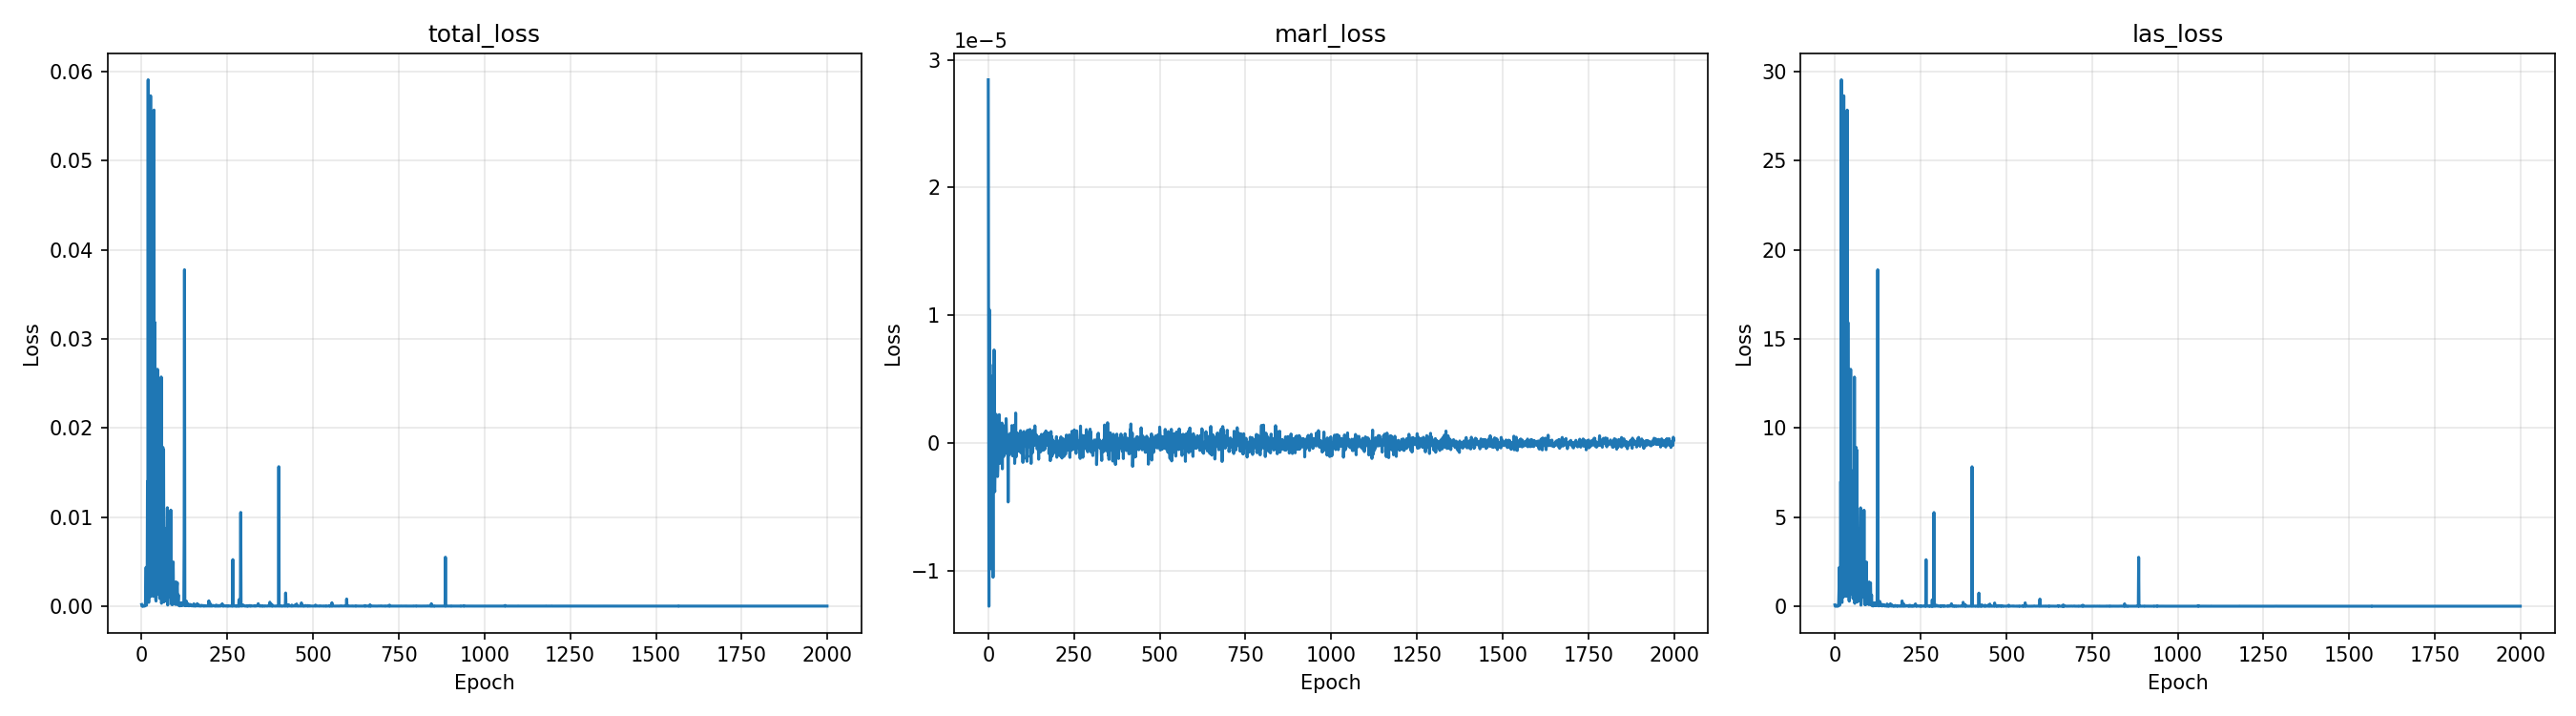
\includegraphics[width=0.98\textwidth]{../graphics/thesis/training_loss_curves.png}
    \caption{训练早期 loss 曲线的局部变化}
    \label{fig:5-2}
\end{figure}

更长时间尺度下的稳定性可由图 \ref{fig:5-3} 观察。可以看到，总损失和 LAS 损失在较长训练区间内保持相对稳定的波动区间，marl\_grad\_norm、las\_grad\_norm 与 total\_grad\_norm 虽随训练推进有逐步抬升趋势，但整体没有出现失控发散。这说明当前的损失权重与训练约束能够维持整体稳定。需要强调的是，loss 稳定并不等于模型已经具备阈值部署能力，因此项目才会把常灰度端点聚集率与训练曲线并列纳入验收标准。

\begin{figure}[H]
    \centering
    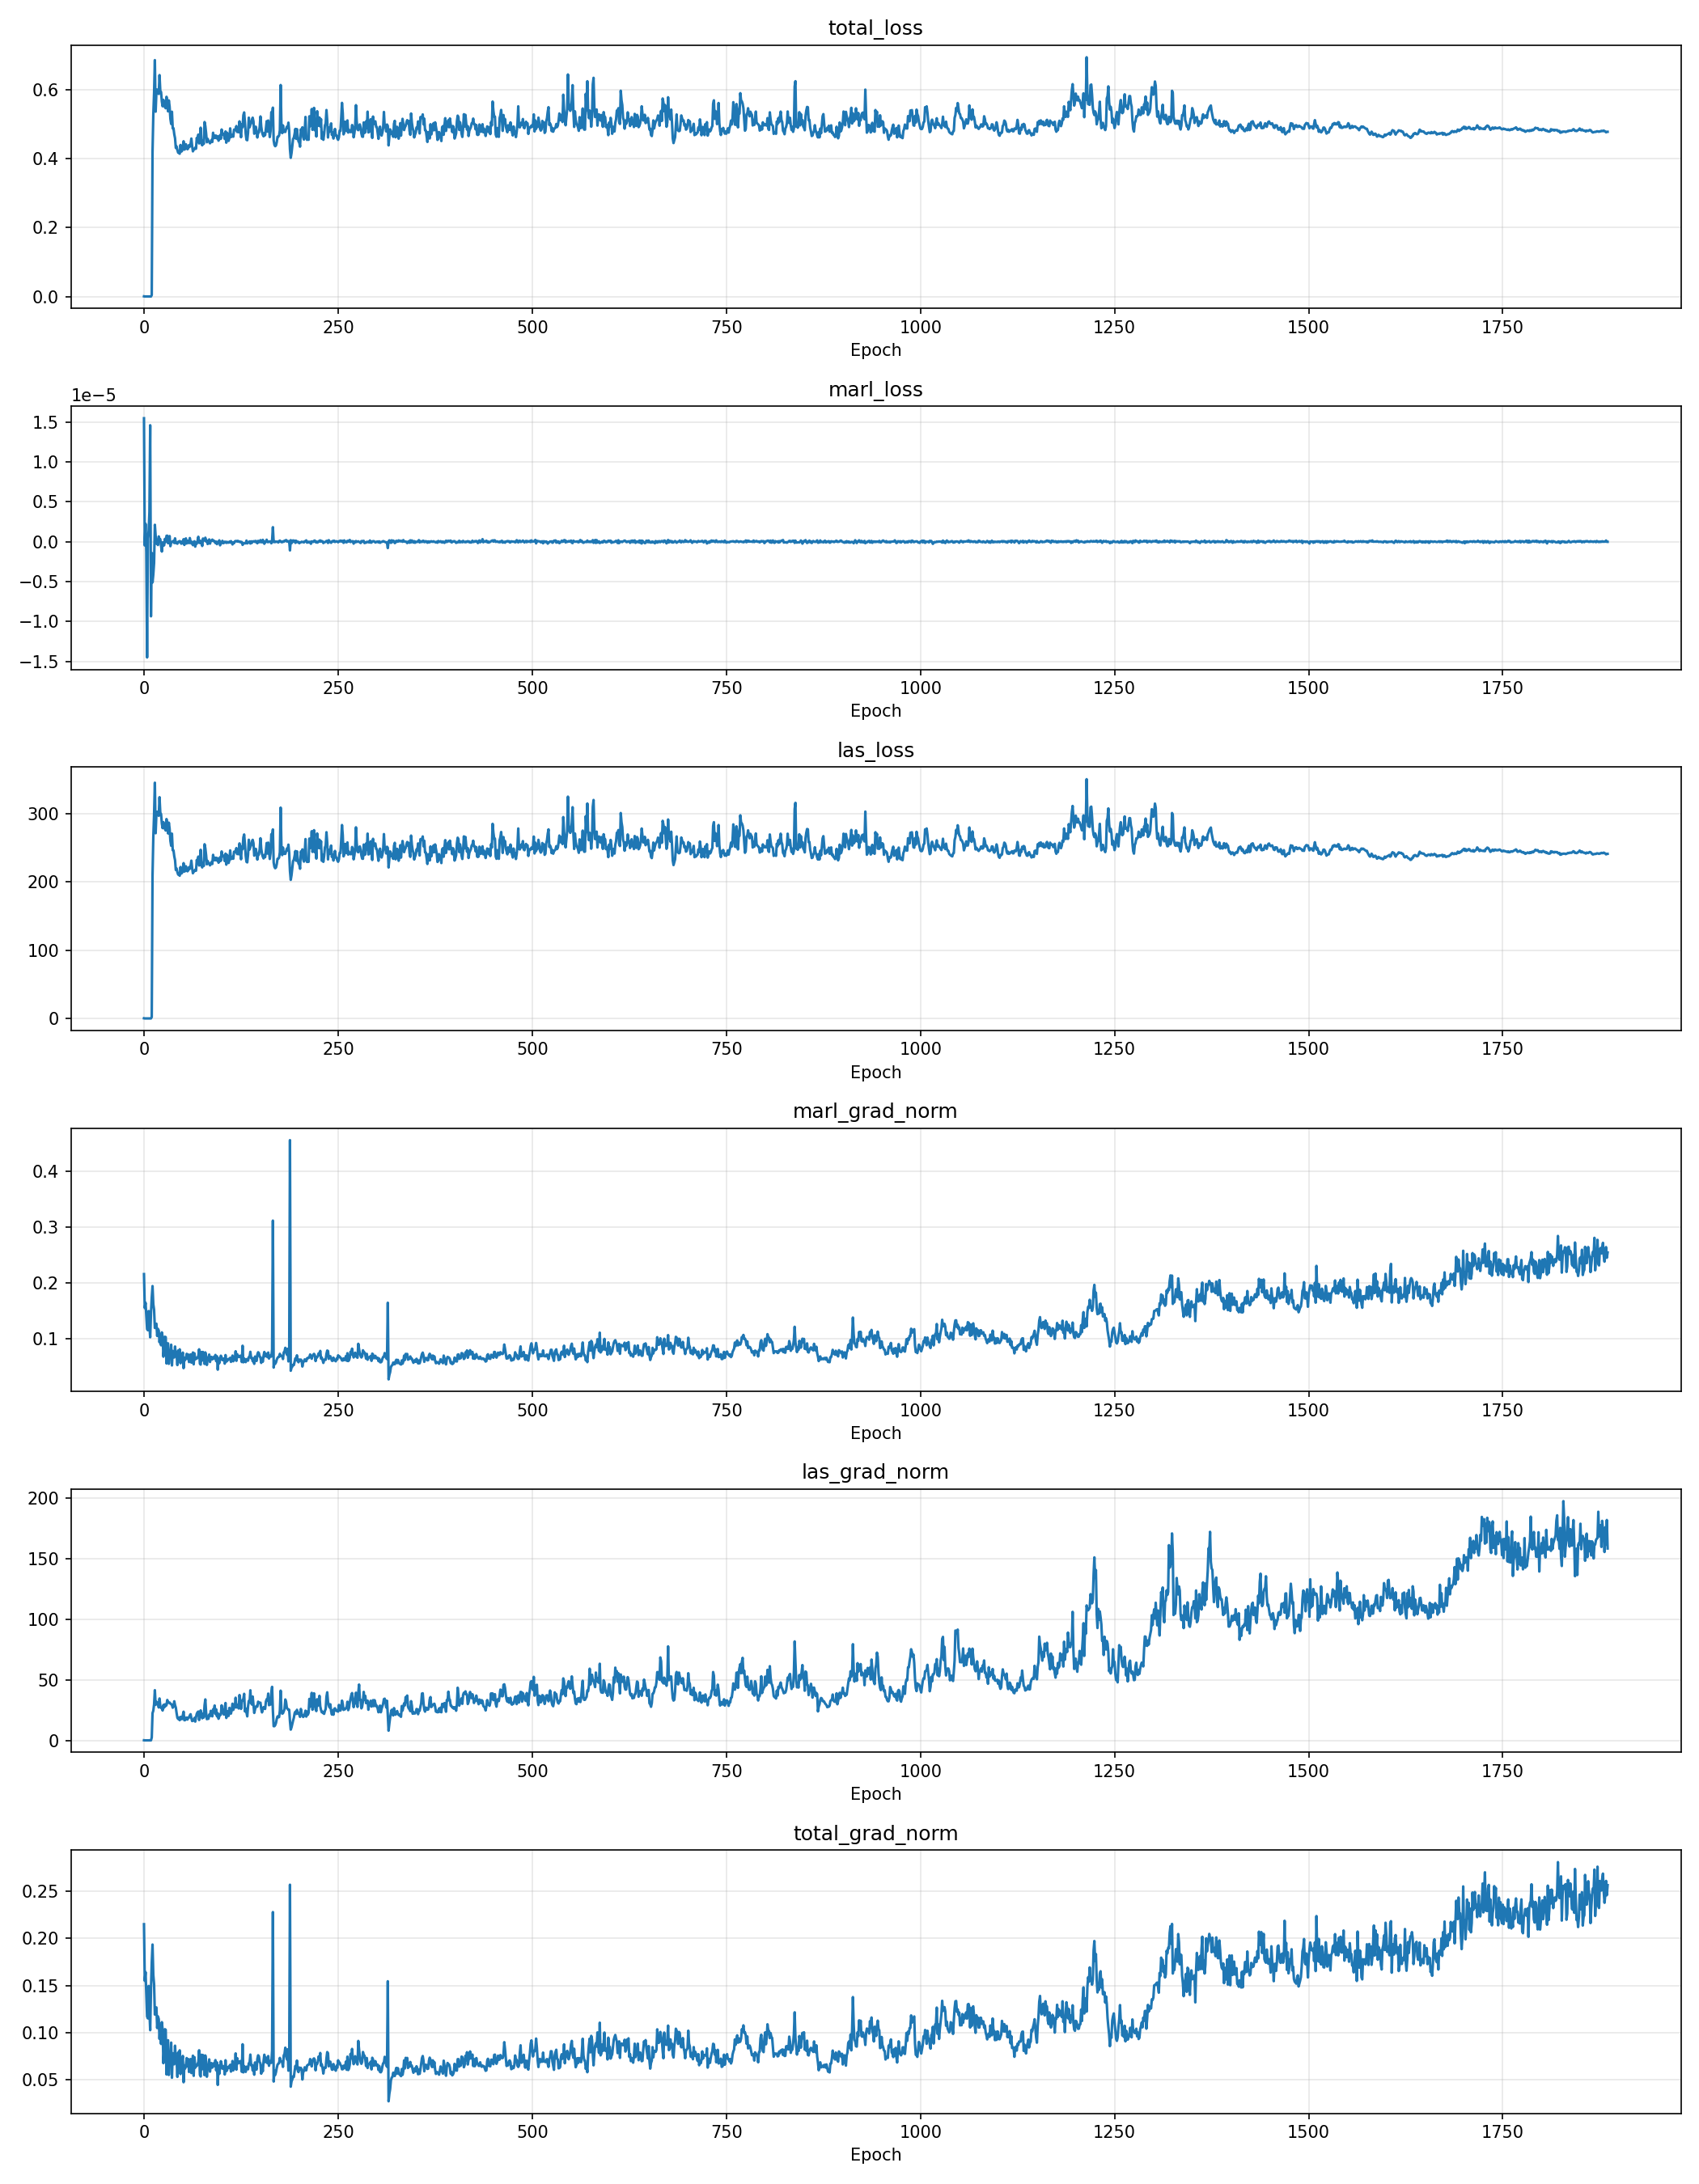
\includegraphics[width=0.98\textwidth]{../graphics/thesis/training_stability.png}
    \caption{训练过程中损失项与梯度范数的整体稳定性}
    \label{fig:5-3}
\end{figure}

在运行效率方面，本文将与主结果同源的运行时归档结果作为正式定量依据。该统计记录了在同一验证流程下执行 20 次预热和 100 次正式统计后的结果：当前模型在 CUDA 环境下处理单张 $512\times512$ 图像的平均耗时约为 12.48 ms，对应约 80.13 张/秒的同尺寸图像吞吐水平。由于该统计与主模型验证结果共享相同的评测口径，因此比临时性的手工测速更适合作为论文正文中的正式报告结果。

另一方面，本文在 AMD Ryzen 7 9700X 与 NVIDIA GeForce RTX 5080 平台上完成了统一基线复评、频谱图生成和正文图表制作。这些补充工作主要用于提高实验章节的完整性和可视化程度，而不与归档主结果混写，以避免不同执行路径、缓存状态或运行模式造成的口径漂移。就方法本身而言，当前模型的核心优势并不在于绝对追求某一种硬件上的极限延迟，而在于它把在线阶段稳定压缩为“一次前向传播 + 固定阈值”的规整流程，从而降低了与现有图像处理链路对接的复杂度。

\begin{table}[H]
    \centering
    \small
    \caption{不同方法的在线计算特征与部署定位比较}
    \label{tab:5-5}
    \begin{tabularx}{0.98\textwidth}{>{\raggedright\arraybackslash}p{0.17\textwidth}>{\raggedright\arraybackslash}p{0.21\textwidth}>{\raggedright\arraybackslash}p{0.12\textwidth}YY}
        \toprule
        方法 & 在线阶段主要操作 & 并行性 & 主要优势 & 主要局限 \\
        \midrule
        Bayer 有序抖动 & 阈值模板查表与逐点比较 & 高 & 在线代价极低，硬件实现简单 & 模板痕迹明显，结构保持能力较弱 \\
        Floyd-Steinberg 误差扩散 & 顺序二值化与量化误差传播 & 中低 & 局部亮度守恒强，感知 PSNR 表现稳定 & 串行依赖明显，不利于大规模并行 \\
        搜索式方法（如 DBS） & 局部翻转/交换与反复误差重计算 & 低 & 视觉质量高，适合离线高质量优化 & 在线迭代代价高，难以实时部署 \\
        本文方法 & 单次卷积前向传播与固定阈值输出 & 高 & 兼顾结构保持、蓝噪声纹理和并行推理 & 仍依赖离线训练，严格感知指标仍有提升空间 \\
        \bottomrule
    \end{tabularx}
\end{table}

表 \ref{tab:5-5} 从在线计算方式出发总结了本文方法与传统路线之间的部署差异。有序抖动仍然是在线阶段最轻量的方案，但其质量上限较低；Floyd-Steinberg 误差扩散在亮度重建方面保持强竞争力，却天然受限于顺序依赖；搜索式方法的主要价值在于离线高质量优化，而不在实时吞吐。相比之下，本文方法通过离线训练换取在线阶段的规整前向计算，因此更适合作为现代并行平台上的高质量预处理模块。

\subsection{目标探针与二值化收敛机理分析}
为了回答“为什么当前模型能够安全阈值化，而 baseline 不能”的问题，项目额外保存了机制探针归档结果。表 \ref{tab:5-3} 对比了 baseline 探针值与最终模型在灰度 0.5 下的关键统计量。可以看到，baseline 的概率均值虽然接近 0.5，但概率标准差只有 0.0129，端点聚集率为 0，阈值白像素比例却跳到 0.7119；相比之下，最终模型的概率标准差提升到 0.4993，端点聚集率达到 0.9969，阈值白像素比例稳定在 0.4989。这说明“采样均值接近目标灰度”并不等价于“模型已经学会可部署的二值策略”。

\begin{table}[H]
    \centering
    \small
    \caption{灰度 0.5 条件下 baseline 与最终模型的关键统计对比}
    \label{tab:5-3}
    \begin{tabular}{lcc}
        \toprule
        指标 & baseline 探针值 & 最终模型值 \\
        \midrule
        概率均值 $\mathrm{prob\_mean}_{g=0.5}$ & 0.5072 & 0.4988 \\
        概率标准差 $\mathrm{prob\_std}_{g=0.5}$ & 0.0129 & 0.4993 \\
        端点聚集率 $\mathrm{endpoint\_ratio}_{g=0.5}$ & 0.0000 & 0.9969 \\
        阈值白像素比例 $\mathrm{threshold\_white}_{g=0.5}$ & 0.7119 & 0.4989 \\
        常灰度平均阈值色调误差 & 0.2824 & 0.0018 \\
        常灰度中灰端点聚集率 & 0.0000 & 0.9954 \\
        \bottomrule
    \end{tabular}
\end{table}

进一步分析灰度 0.5 对应的梯度探针可以发现，熵相关梯度与 MARL 项梯度的余弦相似度为 -0.5570，与混叠抑制相关项梯度的余弦相似度为 -0.7791，二者都指向“把概率推向中间区域”的趋势。这个结果揭示了一个十分重要的事实：仅从局部一阶梯度看，训练目标并不总会自发把概率推向 0 和 1 两端。也正因为如此，常灰度验收集、端点聚集阈值与候选权重筛选在本文方法中并不是可有可无的附加设计，而是弥补局部梯度不足、保证部署稳定性的关键工程机制。

从论文分析角度看，这一探针结果使本文不再只是“汇报好看的指标”，而是能够解释模型为何有效。它表明，当前方法的成功来源于策略建模、感知奖励、辅助频域项和部署导向验收四者的共同作用，而不是某一个单独模块神奇地解决了所有问题。

\subsection{定性案例与失败模式分析}
为补充均值统计，图 \ref{fig:5-4} 和图 \ref{fig:5-5} 展示了两个代表性案例。图 \ref{fig:5-4} 对应室内场景，输入中既包含清晰边缘，也包含较大面积的平坦区域。概率图与阈值结果表明，模型在门框、桌椅轮廓和灯具边缘附近能够形成清晰的结构化黑白分布，而在墙面和地面等大面积平滑区域则通过较均匀的细粒度点阵维持亮度，这体现了策略网络对边缘与背景采用不同纹理密度的能力。

\begin{figure}[H]
    \centering
    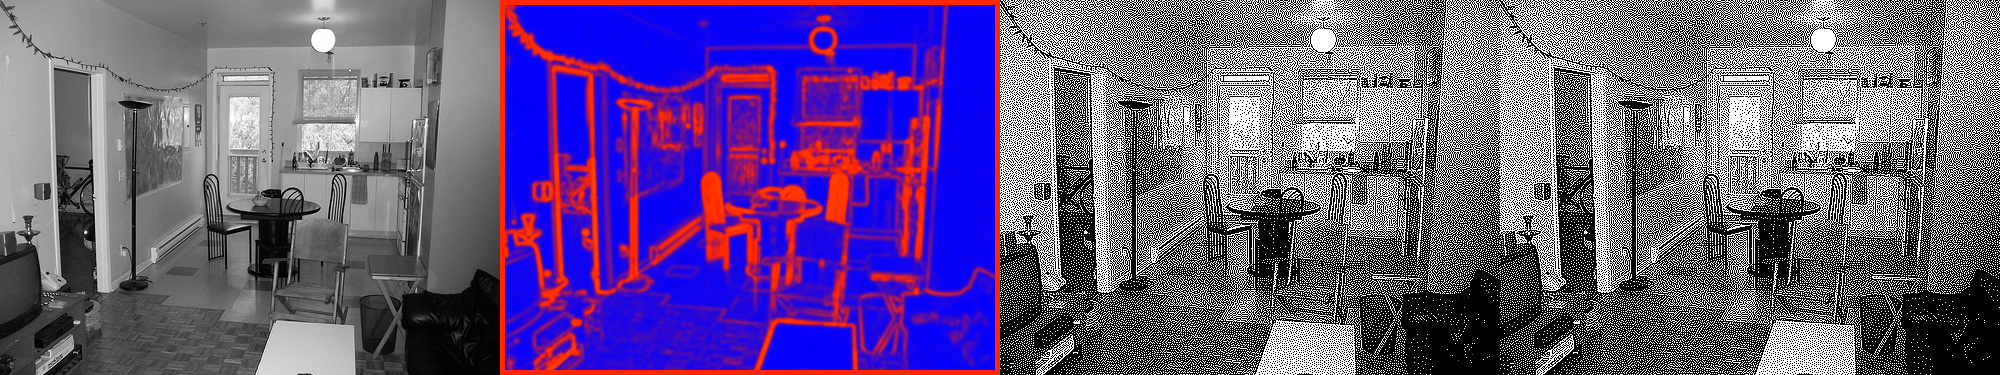
\includegraphics[width=0.92\textwidth]{../graphics/thesis/debug/case_debug_2007_001027.png}
    \caption{代表性案例 1：室内场景中的概率图与阈值结果}
    \label{fig:5-4}
\end{figure}

图 \ref{fig:5-5} 对应演出场景，图像中同时存在强高光、人物轮廓和烟雾状低对比区域。可以看到，模型在主体人物边缘和舞台高光附近能够保留明显结构，但在烟雾和大面积暗背景区域，点阵纹理仍然较强，局部高频扰动比前一案例更明显。这一现象与前文定量分析是一致的：当前模型在主体清晰、局部对比强的区域表现较好，而在复杂纹理与弱对比过渡并存时，感知指标仍会受一定影响。

\begin{figure}[H]
    \centering
    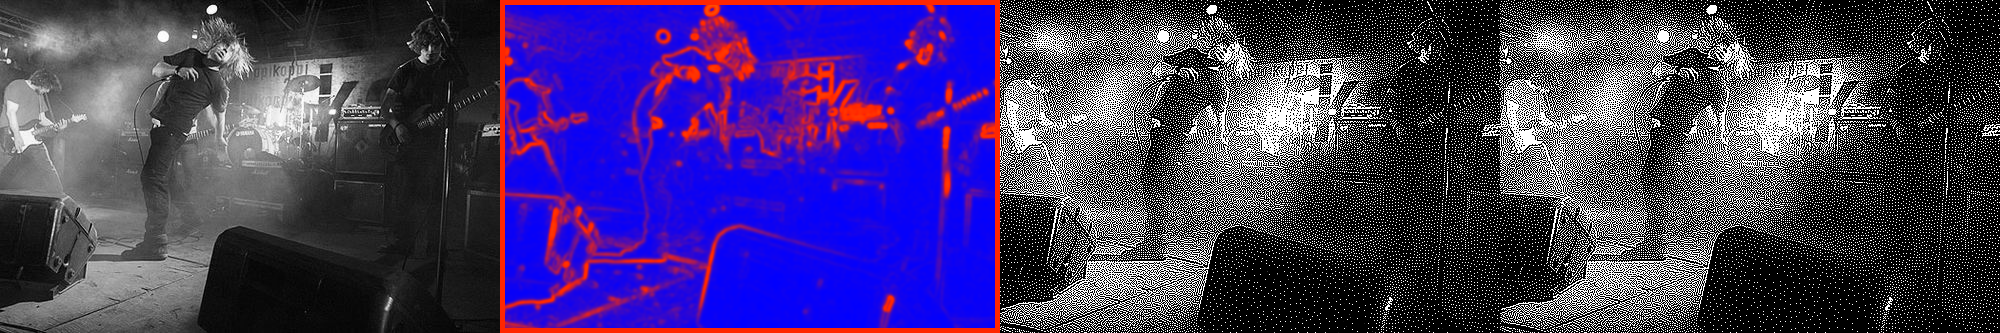
\includegraphics[width=0.92\textwidth]{../graphics/thesis/debug/case_debug_2012_003804.png}
    \caption{代表性案例 2：复杂光照与低对比背景中的概率图诊断}
    \label{fig:5-5}
\end{figure}

结合这些案例，可将当前方法的主要误差来源概括为三类。第一类是大面积低对比背景中的轻微高频噪点，该现象通常不会破坏整体结构，但会拉低严格的感知 PSNR。第二类是弱边缘与缓慢亮度过渡区域中的阈值敏感性，当局部概率接近 0.5 时，固定阈值可能引起比采样输出更强的亮度偏差。第三类是复杂纹理和显著结构边缘并存时的双重约束冲突，即模型既要保留主体轮廓，又要维持蓝噪声特性，二者有时难以同时达到最优。

\subsection{常灰度分段机制分析}
前文已经从整体平均角度说明了常灰度 suite 的有效性，但若要进一步解释模型为何具备可部署的二值化能力，还需要把不同灰度区间拆开分析。原因在于，低灰度区域、中灰度区域和高灰度区域在纹理组织上的任务并不相同：低灰度强调稀疏白点的稳定生成，中灰度强调双峰概率分布和蓝噪声均衡，高灰度则更接近对白底稀疏黑点分布的对称控制。分段分析能够把这些差异显式写出来，从而让实验讨论从“有结果”提升到“有机制”。

\subsubsection{低灰度区域的稀疏白点分布规律}
在低灰度区域，模型的关键任务是在大面积黑背景中稳定地产生稀疏白点。对灰度 0.1 的常值输入，最终模型的概率均值为 0.0984，概率标准差为 0.2968，端点聚集率达到 0.9974，阈值白像素比例为 0.0984，阈值色调误差仅为 0.0016。灰度 0.2 时，概率均值为 0.1959，概率标准差增至 0.3958，端点聚集率为 0.9963，阈值白像素比例为 0.1959，阈值色调误差约为 0.0041。上述结果表明，模型并没有依赖大量处于中间状态的概率值去“凑出”正确均值，而是已经能够在低灰区域形成稳定的端点化稀疏点分布。

这一点在与 baseline 对照时更加明显。机制探针归档结果显示，baseline 在灰度 0.2 下的概率均值仅为 0.1725，概率标准差只有 0.0099，端点聚集率为 0，阈值白像素比例更是直接降到 0。也就是说，如果模型停留在 baseline 状态，那么部署阶段一旦采用固定阈值，低灰度区域几乎会完全丢失应有的白点，导致整体偏暗失真。最终模型能够把这一现象纠正过来，说明常灰度验收和端点收敛机制对低灰区域尤其重要。

从频域角度看，低灰度区域也提供了一个观察方向性纹理是否过强的窗口。灰度 0.1 和 0.2 对应的阈值各向异性值分别约为 0.2423 dB 和 0.4083 dB，虽然高于中灰区域，但仍处于可接受范围内，没有表现出明显的条纹化趋势。这说明模型在稀疏点分布场景下并未通过聚团或规则栅格去完成色调近似，而是仍尽量维持较均匀的随机排布。

\subsubsection{中灰度区域的端点收敛与阈值稳定性}
中灰度区域通常是半色调任务中最具判别性的部分，因为它既要求白点与黑点高度混合，又要求大尺度亮度不偏移。灰度 0.4 时，模型的概率均值为 0.3971，概率标准差为 0.4880，端点聚集率达到 0.9946；灰度 0.5 时，概率均值为 0.4988，概率标准差升至 0.4993，端点聚集率达到 0.9969，阈值白像素比例稳定在 0.4989；灰度 0.6 时，概率均值为 0.5999，概率标准差为 0.4887，端点聚集率为 0.9946。这组结果清楚表明，模型在中灰区域并没有停留在“所有像素都接近 0.5”的模糊中间态，而是把概率质量有效推向两端，再通过空间比例控制整体亮度。

与此形成鲜明对比的是 baseline 在灰度 0.5 下的表现。虽然其 sample\_white 仍接近 0.5048，但 prob\_std 只有 0.0129，endpoint\_ratio 为 0，threshold\_white 却跃升到 0.7119，gray\_threshold\_sample\_gap 高达 0.2072。这说明单纯依赖采样结果，很容易误以为模型已经“学会”中灰半色调；但只要切换到固定阈值部署，问题就会立刻暴露。最终模型将灰度 0.5 下的 threshold\_sample\_gap 压到约 0.0001，正是端点收敛真正完成的标志。

中灰区域同时也是观察蓝噪声特性的最佳窗口。以灰度 0.5 为例，采样结果与阈值结果的各向异性值分别为 0.0059 dB 和 0.0128 dB，二者都已接近各向同性；对应的高频混叠能量也都约为 0.3116。虽然这并不能说明模型已经达到理论最优蓝噪声，但至少表明它在最难的中灰区域没有形成明显方向条纹，也没有因过度追求端点聚集而破坏频谱均衡性。对于论文而言，这部分讨论比单纯重复均值更有解释力。

\subsubsection{高灰度区域的对称性与频谱趋势}
高灰度区域可以被看作低灰区域的对偶问题。灰度 0.7 时，模型的概率均值为 0.7006，端点聚集率为 0.9956，阈值白像素比例为 0.7006；灰度 0.8 时，概率均值为 0.8016，端点聚集率为 0.9956，阈值白像素比例为 0.8016；灰度 0.9 时，概率均值为 0.9024，端点聚集率达到 0.9952，阈值白像素比例为 0.9023。可见模型并未在亮区域出现系统性饱和偏差，而是能够对白底上的稀疏黑点进行较稳定控制。

从频域指标看，随着灰度从 0.5 上升到 0.9，阈值混叠能量从约 0.3116 下降到 0.0212。这一趋势是可以理解的：在更高灰度下，黑点数量越来越少，可组织的高频结构密度随之下降，因此高频别名能量自然降低。更重要的是，这一变化趋势与视觉直觉一致，并没有出现反常的高频尖峰。与此同时，灰度 0.7、0.8、0.9 对应的阈值各向异性值分别约为 -0.0522 dB、0.2350 dB 和 -0.0471 dB，整体仍处于较小范围内，说明模型即使进入稀疏黑点场景，也没有形成强烈方向偏置。

对比 baseline 在灰度 0.8 下的行为，这种改进更加明显。baseline 的 threshold\_white 会直接饱和到 1.0，意味着固定阈值部署后高灰区域完全失去稀疏黑点结构，只剩纯白块状区域；而最终模型则能把 threshold\_white 保持在 0.8016 左右，并维持较合理的频域统计。这说明当前方法并非只在中灰区域有效，而是在整个灰度范围内都形成了相对一致的二值决策规律。

\subsubsection{从分段结果回看训练闭环}
把低灰度、中灰度和高灰度的结果放在一起观察，可以更完整地理解当前训练设计的有效性。低灰区域强调“稀疏白点不能消失”，中灰区域强调“概率必须双峰化”，高灰区域强调“稀疏黑点分布要与低灰对称”。如果模型在任意一区间失败，常灰度 suite 的整体端点聚集率、阈值色调误差和 threshold\_sample\_gap 都会明显恶化。因此，这组分段结果实际上反向证明了当前的主奖励、辅助损失和验收阈值是共同起作用的，而不是某个灰度档位上的偶然成功。

这也是为什么本文把常灰度 suite 视为比单一自然图像样例更重要的机制证据。自然图像容易受到语义内容、边缘强度和纹理复杂度影响，而常灰度图像几乎剥离了这些因素，只保留“模型如何组织二值纹理”这一核心问题。对本科毕业论文而言，把这条逻辑写清楚，能够显著增强实验章节的深度与说服力。

\subsection{训练目标、部署目标与证据链讨论}
在许多深度视觉任务中，训练目标和部署目标往往高度一致，例如分类任务直接优化类别预测，连续回归任务直接优化数值误差。但半色调并不完全符合这一模式。训练阶段允许模型输出概率图，并通过采样维持期望上的正确白像素比例；部署阶段却更希望得到稳定、可重复且低延迟的硬阈值输出。这意味着“训练时看起来合理”和“部署时真正可用”并不是同一个条件。

本文之所以把常灰度端点聚集率、采样-阈值差值和目标探针放到核心位置，正是为了显式处理这一差异。以灰度 0.5 为例，最终模型的采样-阈值差值仅约 0.0001，而 baseline 高达 0.2072。这说明前者在采样和阈值两种输出方式之间几乎没有统计裂缝，后者则存在明显的部署断层。对论文而言，这一事实非常关键，因为它把“端点收敛”从隐含假设转变为可量化、可讨论、可验收的研究对象。

围绕这一问题，本文的证据链可以概括为三个层次。第一层是候选测试集均值和小规模整图结果，它们回答“模型总体效果是否成立”；第二层是常灰度 suite 和分段分析，它们回答“模型是否在整个灰度范围内形成稳定二值策略”；第三层是目标探针与运行时统计，它们回答“为何该策略能够部署，以及部署成本是否可接受”。当这三层证据被统一组织后，论文结论就不再只是数字列表，而是具有明确指向的问题链条。

为避免实验讨论在后续小节中反复回收相同结论，表 \ref{tab:5-6} 对本章最关键的研究问题、对应证据与工程含义作进一步汇总。这样处理的目的不是用一张表代替前文分析，而是先把“结论骨架”明确下来，再让读者回看各小节中的指标、案例图和机制解释，从而降低实验章节的信息分散度。

\begin{table}[H]
    \centering
    \small
    \caption{本章核心结论、证据来源与工程含义汇总}
    \label{tab:5-6}
    \setlength{\tabcolsep}{4pt}
    \begin{tabularx}{0.98\textwidth}{>{\raggedright\arraybackslash}p{0.18\textwidth}>{\raggedright\arraybackslash}p{0.24\textwidth}>{\raggedright\arraybackslash}p{0.20\textwidth}X}
        \toprule
        研究问题 & 主要证据来源 & 直接结论 & 工程含义 \\
        \midrule
        自然图像总体质量是否成立 & 候选测试集主结果、小规模整图补充结果、统一基线复评 & 本文方法在 CSSIM 和 SSIM 上占优，Gaussian-HVS PSNR 接近目标均值，但 Nasanen-HVS PSNR 仍有提升空间 & 方法已经具备自然图像上的总体可用性，但现阶段不能宣称在所有感知指标上全面超过经典误差扩散 \\
        固定阈值部署是否稳定 & 常灰度验收结果、表 \ref{tab:5-2}、灰度分段分析 & 整体端点聚集率达到 0.9957，阈值色调误差仅 0.0018，中灰区域已经形成双峰概率分布 & 模型不再依赖在线采样维持视觉效果，可以作为固定阈值半色调模块部署 \\
        端点收敛为何不是自然发生 & 表 \ref{tab:5-3}、灰度 0.5 目标探针 & baseline 虽能采样出近似均值，但阈值输出严重失真；最终模型则把采样与阈值之间的差值压到近 0 & 常灰度验收与候选模型筛选属于必要机制，而不是附属可视化步骤 \\
        在线推理是否具备工程潜力 & 运行时归档、表 \ref{tab:5-5}、整图推理流程 & 在 CUDA 环境下，$512\times512$ 单图平均耗时约为 12.48 ms，在线阶段退化为一次前向传播与固定阈值 & 方法更适合 GPU 批处理场景，其速度优势不宜直接外推到 CPU-only 场景 \\
        \bottomrule
    \end{tabularx}
\end{table}

从本科毕业论文的写作角度看，这张汇总表还有一个作用，即把“结果成立”“机制可解释”“部署可落地”三类结论明确拆开。这样一来，后文即使继续讨论部署约束、评价指标互补关系或实验复现流程，也都可以回收到表 \ref{tab:5-6} 所对应的问题框架中，而不会演变成简单的材料堆积。

\subsection{与实际打印链路的衔接及扩展场景}
从系统接口看，当前方法位于打印或显示预处理链路中的“高质量二值图生成”阶段。其输入为连续调灰度图，输出为同尺寸二值半色调图，因此可以较自然地嵌入图像读取、灰度预处理、设备适配和缓存输出之间。由于当前推理流程已经实现 halo padding 与回裁，理论上也能够以分块方式处理大尺寸图像，再将各块结果拼接回完整版面，这一点对高分辨率打印场景尤其重要。

与传统误差扩散相比，本文方法更适合作为批处理或服务化推理模块部署。离线训练完成后，在线阶段只需准备输入图像和噪声图，即可一次性得到概率图和阈值结果。若后续业务更强调结果一致性，可以固定噪声模板或直接使用确定性阈值输出；若处理超大幅面图像，则可以结合当前已有的分块推理接口组织整图流程。当前实现尚未把这些部署策略全部扩展为独立产品级功能，但其接口已经相对清晰。

需要注意的是，真正进入实际打印链路后，还会出现点增益、纸张吸墨、观察距离变化和设备分辨率差异等问题，这些因素都会改变最优半色调纹理。当前论文能证明的是该方法在数值实验和图像观察层面具备较好潜力，而不是已经解决所有设备侧适配问题。因此，CPU-only 评测、量化推理、介质建模和设备校准仍属于后续工程化的重要环节。

从扩展场景看，灰度二值半色调可以被视作更一般离散输出问题的起点。若目标设备支持多级墨量输出，则每个像素的动作空间可以从伯努利分布扩展为多项分布；若目标是彩色半色调，则还需要同时控制跨通道之间的综合色差和频域串扰。这些问题在本文中尚未展开系统实验，但当前的强化学习建模和验收思路为后续扩展提供了可沿用的框架基础。

\subsection{评价指标的互补关系与场景适配}
半色调任务需要同时考察结构保真、亮度还原、频谱分布和部署稳定性四类问题，因此本文联合使用 CSSIM、SSIM、两类 HVS-PSNR、各向异性值、混叠能量和端点聚集率等指标。CSSIM 与 SSIM 主要回答主体结构是否得到保留，Gaussian-HVS PSNR 与 Nasanen-HVS PSNR 主要反映观察尺度下的亮度误差，各向异性值和混叠能量用于描述蓝噪声频谱，端点聚集率则直接检验概率图能否安全阈值化。只有把这些问题放在一起讨论，才能较完整地评价一套半色调方法。

为使这些指标之间的分工更加清晰，表 \ref{tab:5-4} 对各类指标的关注对象和使用场景作了归纳。表中可以看出，本文并没有刻意让不同指标相互重复，而是把它们组织成从“主观感知”到“频域性质”再到“部署可行性”的递进结构。这样的组织方式有助于避免在实验讨论中把结构保真、蓝噪声质量和二值稳定性混为一谈。

\begin{table}[H]
    \centering
    \small
    \caption{本文主要评价指标及其作用分工}
    \label{tab:5-4}
    \begin{tabularx}{0.98\textwidth}{>{\raggedright\arraybackslash}p{0.18\textwidth}YYY}
        \toprule
        指标 & 主要关注对象 & 适合回答的问题 & 使用时需注意的限制 \\
        \midrule
        CSSIM & 局部结构与对比敏感区域 & 主体轮廓和细节是否仍易辨认 & 不能单独说明频谱是否合理 \\
        SSIM & 一般结构相似性 & 与传统结构指标的可比性如何 & 在噪声纹理较多时解释力有限 \\
        Gaussian-HVS PSNR & 平滑观察尺度下的亮度误差 & 整体色调是否稳定 & 对更严格视觉模型的约束不如 Nasanen \\
        Nasanen-HVS PSNR & 更严格的人眼低通观察误差 & 在严格感知条件下是否仍接近原图 & 对局部纹理扰动更敏感 \\
        各向异性值 & 频谱方向均衡性 & 是否出现方向性条纹或结构化噪声 & 不能替代亮度和结构指标 \\
        混叠能量 & 高频区域异常能量聚集 & 高频纹理是否存在尖峰伪影 & 需要结合灰度区间解释变化趋势 \\
        端点聚集率 & 概率输出双峰化程度 & 模型能否安全阈值化部署 & 不能单独说明主观视觉质量 \\
        \bottomrule
    \end{tabularx}
\end{table}

当前结果之所以具有说服力，正是因为这些指标大多指向同一结论，而不是彼此冲突。若只有 CSSIM 较高但端点聚集率较低，模型很可能只是学会了一个连续概率图；若只有各向异性值较优但 HVS-PSNR 较差，则说明纹理频谱虽然接近蓝噪声，但主体亮度或结构并未被有效保留。本文方法在候选测试集、常灰度 suite 和目标探针三个层面上都能取得较为一致的结论，因此可以认为当前改进不是单一指标上的偶然过拟合，而是较为完整的综合提升。

从具体图像场景看，不同指标的敏感性也并不相同。对于主体边缘清晰、局部对比强的图像，CSSIM 和 Gaussian-HVS PSNR 通常更容易给出积极反馈，因为这类场景的结构信息明确，策略网络更容易在边缘附近形成稳定二值排列。对于天空、墙面、雾景或阴影等低对比平坦区域，端点聚集率、threshold\_sample\_gap 和灰度误差往往更具解释力，因为这些区域最容易暴露“采样尚可、阈值失真”的问题。对于植被、毛发、织物和远景建筑等细密重复纹理场景，各向异性值、混叠能量与严格 HVS-PSNR 的变化则更值得关注，因为这些区域最容易出现方向性噪声或局部高频伪影。

换言之，本文并没有试图通过单一指标给出“最终判决”，而是把不同指标放回各自最擅长解释的问题域中。这样处理虽然会让实验章节更长，但能显著提高论证质量，也更符合本科毕业论文对完整性和严谨性的要求。

\subsection{实验复现、归档与证据链组织}
在多指标、多图像和多类结果文件并存的情况下，论文最容易出现的问题不是证据不足，而是证据碎片化。为避免这一问题，本文在组织实验讨论时始终遵循“整体结果、机制解释、部署条件”三层递进关系，并把每一层结论都锚定到可追溯的文件或图像上。与其把所有数字堆在同一张表里，不如先明确每种证据分别服务于什么问题，再讨论它们之间如何互相支撑。

\subsubsection{复现流程的层次化组织}
从当前实现的真实工作流来看，较合理的复现顺序并不是“先跑所有图像，再事后解释”，而是先完成常灰度验收，再做整图验证，最后补充机制探针和运行时测量。训练阶段首先需要通过常灰度验收集确认模型已经离开中间概率状态；随后在小规模整图验证样本上做快速一致性检查，观察主体边缘是否存在明显偏差；接着再在 1684 张候选测试图像上统计整图均值；最后利用机制探针结果和运行时统计补充机制与效率证据。这样的顺序能够有效降低无效实验的规模，也更符合实际工程调试逻辑。

对论文写作而言，这种层次化组织同样重要。若直接从候选测试集均值开始，读者很容易把结论理解为“模型效果还行”；但若先展示常灰度验收，再引入目标探针，就能更清楚地说明模型为什么不仅“看起来可用”，而且“阈值部署后仍然可用”。这也是本文实验章节比普通结果汇总更长的原因，因为它不仅关心结果大小，更关心结果的来源和意义。

\subsubsection{结果文件的角色分工}
主统计归档结果负责回答总体表现问题。它同时包含大规模候选测试集、小规模整图验证样本和常灰度验收集三类结果，使自然图像质量、主结果目标差距和常灰度统计能够在同一处统一管理。对于论文而言，这类归档结果相当于总账本，用来支撑表 \ref{tab:5-1}、表 \ref{tab:5-2} 以及常灰度分段分析中的大部分数值。

机制探针归档结果的角色则更偏向机制解释。它记录 baseline、最终模型和灰度 0.5 附近的梯度探针结果，用于回答“为什么某些目标项会把概率往中间拉回去”“为什么采样均值正确仍然可能导致阈值部署失败”以及“为什么必须把端点聚集率单独纳入验收”这类问题。若没有这类归档结果，论文很容易停留在经验性描述层面，而难以说明训练闭环为什么必要。

运行时归档结果的功能相对直接，但同样不可或缺。它把预热轮数、正式统计轮数和平均耗时明确记录下来，使效率结论不再只是口头判断，而有了可复核的统计口径。对于一篇强调工程落地潜力的本科毕业论文而言，这类结果虽然简单，却能有效弥补“只讲质量不讲成本”的缺口。

\subsubsection{从训练日志到论文论点的映射}
训练日志不仅记录数值变化，也暗含了不同阶段的模型行为。早期阶段，总损失和 LAS 损失尖峰较多，说明模型仍在快速适应亮度和纹理的联合约束；中期阶段，主损失趋稳而梯度范数缓慢抬升，意味着网络开始在较稳定的感知质量基础上微调蓝噪声特性；后期阶段，若端点聚集率持续升高并趋于稳定，则可以推断概率输出已经逐步完成双峰化。这种阶段性解读对于半色调任务尤为重要，因为模型是否进入“可阈值化状态”并不能只靠一条单独损失曲线判断。

因此，本文在论述训练过程时并没有把日志简单视为附录材料，而是把它看作方法有效性的动态证据。图 \ref{fig:5-2} 和图 \ref{fig:5-3} 负责呈现训练过程的整体趋势，而常灰度分段分析和目标探针则负责把这些趋势转译为更具语义的结论。二者结合后，训练章节才能真正形成“过程--状态--结论”的完整链条。

\subsubsection{证据链如何支撑论文结论}
从整篇论文的组织方式看，候选测试集均值、常灰度 suite、目标探针、案例图像和运行时统计并不是相互平行的材料，而是构成了一条逐层收紧的证据链。第一层用整图均值说明方法具有总体有效性；第二层用常灰度统计说明方法在整个灰度范围内形成稳定的二值纹理；第三层用目标探针说明这一稳定性并不是训练目标自然赠送的，而是验收闭环与辅助设计共同实现的；第四层用案例图与运行时文件说明这种能力既有视觉表现，也具备一定工程潜力。

这样的证据链组织方式还有一个额外好处，即它能自然容纳“不足”和“结论边界”。例如，当本文指出 Nasanen-HVS PSNR 与目标均值仍有差距时，这一现象可以被放回第一层整体结果中理解；当本文指出低对比背景中仍存在轻微高频扰动时，这一现象可以被放回第二层与第四层之间的联系中理解；当本文指出尚未完成统一基线对比时，这一问题又可以被放回证据链的边界条件中解释。换言之，证据链不仅支持结论，也帮助界定结论的适用范围。

\subsection{工程部署约束与扩展路径分析}
尽管当前方法已经在 CUDA 环境下展示出较好的推理效率，但真正进入工程部署阶段时，仍需要面对一系列比论文实验更细碎也更现实的约束。首先是算力平台差异。当前 12.48 ms 的结果基于 GPU 前向推理，而工业链路中并不总能提供同等级别的并行硬件。若部署目标转向 CPU-only 或资源受限的主控芯片，那么轻量网络本身虽提供了良好基础，但仍需进一步结合量化、剪枝、蒸馏或更小通道数配置，才能把实验室环境中的速度优势转化为稳定的端侧收益。

第二个约束来自大幅面图像处理方式。打印任务往往涉及远大于 $512\times512$ 的输入尺寸，若直接整图推理，显存和带宽压力都会快速增加。当前推理流程通过自动估计感受野半径和 halo padding，为分块推理提供了良好前提：可以将大图拆分为若干带 halo 的局部块，在保证边界一致性的前提下分别前向计算，再拼接成最终结果。这意味着系统并不需要彻底重写，便可向更实际的大尺寸处理链路靠近；但与此同时，块间噪声一致性、I/O 调度和流水线吞吐仍需要更细致的工程测试。

第三个约束来自纹理随机性与业务可控性之间的平衡。由于策略网络输入包含随机噪声图，不同噪声实例可能带来细粒度纹理差异。从研究角度看，这种随机性是蓝噪声多解性的重要来源；但从工程角度看，某些场景可能更希望同一输入始终得到完全一致的输出。对此，后续部署可以考虑固定噪声模板，或在策略充分收敛后改用确定性阈值输出，从而在纹理多样性与结果一致性之间做更明确的取舍。本文当前结果已经表明，模型在端点收敛后具备较强的阈值稳定性，因此这类控制策略具备实现基础。

第四个约束来自打印介质和设备物理特性。半色调结果在真实设备上还会受到点增益、纸张吸墨、分辨率、喷头排列和观察距离等因素影响。当前论文中的 HVS 评价和频谱分析主要解决“图像层面的可感知质量”，而非“设备层面的最终物理表现”。因此，若要进一步推动工程落地，除了继续优化网络本身，还需要结合设备响应模型和打印介质特性做更完整的链路校准。这也是本文在部署结论上保持克制的原因，即它证明了方法具有潜力，但并未宣称已经完成全部工业适配。

从扩展路径看，本文方法最值得保留的并不是某个固定指标，而是其整体框架的可迁移性。状态、动作、奖励、灰度验收和证据链组织这些核心思路，都可以迁移到彩色半色调、多级输出设备甚至其他离散图像生成任务中。换言之，当前灰度二值半色调研究既是一个具体问题的阶段性结果，也可以被视作更一般离散感知优化问题的出发点。

\subsection{研究贡献、结论边界与学术价值讨论}
若从论文整体结构回看，本文完成的核心工作，是把一套强化学习半色调实现系统化地组织为一条较完整的研究链条。第一，本文明确指出半色调任务的核心难点不只是生成黑白点阵，而是同时处理色调统计、蓝噪声频谱、离散动作优化和部署阶段阈值稳定性。第二，本文把单步多智能体强化学习方案系统化地表达出来，使状态、动作、奖励、策略网络、常灰度验收和目标探针之间的关系在论文中形成清晰闭环。第三，本文把代码输出、结构化结果文件和定性图像组织为证据链，使实验结论具备可追溯性而非仅凭叙述成立。

从研究贡献的强度上看，本文不应被夸张描述为“提出了全新的通用半色调理论”，但完全可以合理地表述为：在一个具体而重要的灰度半色调问题上，完成了强化学习建模、轻量网络实现、部署导向验收和实验组织方式的系统整合。对本科毕业论文而言，这样的贡献定位是扎实且可信的。它既体现了对图像处理、深度学习和工程实现的综合把握，也避免了超出证据边界的过度包装。

同样需要强调的是，结论边界并不等于工作价值不足。当前论文没有统一重跑所有传统基线，没有完成彩色场景验证，也没有引入真实打印设备侧标定，这些都属于明确存在的空缺；但这并不妨碍本文在“灰度半色调的离散策略学习及其部署可行性”这一问题上给出较完整的回答。事实上，主动说明边界反而有助于提高论文可信度，因为它表明研究者清楚哪些结论来自已验证结果，哪些仍属于下一阶段工作。

从学术价值看，本文至少提供了两点值得保留的认识。其一，在半色调这类离散输出任务中，采样可行并不等于阈值可部署，必须显式检查概率图是否真正完成端点收敛；其二，实验章节的质量不仅取决于数字是否漂亮，也取决于结果、机制和部署证据是否能够互相支撑。这两点认识虽然看似朴素，却直接关系到很多工程型研究能否从“跑通代码”提升到“形成论文论证”。

因此，本文的学术价值并不只体现在某个指标数值，而体现在一种较为完整的研究和写作范式：先从任务本质确定控制问题，再围绕这些问题组织代码、实验和结果，最后用多层次证据链回收结论和边界。对于本科毕业设计而言，这样的范式本身就具有方法论意义，也为后续更严格的实验和更复杂的任务扩展留下了清晰接口。

\subsection{与传统方法的比较和研究定位}
本文补充的统一基线实验虽只覆盖 Bayer 有序抖动和 Floyd-Steinberg 误差扩散两类可直接复现的传统方法，但其结果已经足以帮助定位当前方法。可以看到，Bayer 有序抖动在统一协议下整体落后，而 Floyd-Steinberg 仍保持很强竞争力，尤其在两类 HVS-PSNR 上优于本文方法。这说明经典误差扩散在观察尺度亮度保真方面依然具有难以忽视的优势。

与此同时，本文方法的定位也因此变得更加清楚：它的优势不在于“全面替代所有传统算法”，而在于在一次前向并行推理、较高 CSSIM/SSIM、近零 dB 各向异性以及端点收敛证据链之间取得更稳定的综合折中。误差扩散仍然适合无需训练、强调 CPU 直接部署的场景；Bayer 有序抖动适合极端轻量和高吞吐链路；本文方法则更适合已经具备 GPU 或批处理环境、同时希望兼顾结构保持、蓝噪声特性和部署一致性的场景。对本科论文而言，明确这一定位比笼统宣称“优于传统方法”更重要。

\subsection{有效性威胁与结论边界}
为了避免结论表述过度，本文需要明确若干有效性威胁。首先，本章大量定量结果来自项目已经保存的结果文件，而非本次写作阶段重新从零完整复训得到，因此论文结论建立在原训练过程稳定、结果归档可信的前提下。其次，当前运行时数据仅覆盖 CUDA 环境下的 $512\times512$ 单图推理，不能直接外推为 CPU 平台或更大分辨率场景的最终表现。再次，本文虽已补充统一口径下的 Bayer 有序抖动和 Floyd-Steinberg 误差扩散对照，但尚未纳入 DBS、SAED 等更强搜索式或结构感知型基线，因此有关“与全部经典方法的全面比较”仍不能视为已经完成。

此外，当前研究对象仍以灰度半色调为主，对彩色场景、多级输出设备、实际纸张介质点增益以及跨设备泛化问题尚缺乏系统实验。换言之，本文真正证明的是：在当前实现、当前数据划分和当前归档结果范围内，强化学习驱动的轻量级卷积策略网络已经表现出较好的结构质量、蓝噪声特性与在线效率；但若要将其推广到更复杂场景，还需要补充更完整的实验链条。

\subsection{本章小结}
本章围绕主结果、常灰度行为、训练稳定性、目标探针、定性案例与方法定位，对当前模型进行了较系统的论证。实验表明，模型已经在 CSSIM、Gaussian-HVS PSNR、端点聚集率和推理效率等方面取得较均衡表现，同时也暴露出在更严格感知指标、复杂背景场景和统一基线对比上的进一步提升空间。更重要的是，本章说明了这些结果为何可信，以及它们在何种边界内成立，从而使论文的实验部分具备了较完整的解释力。

\section{总结}

\subsection{研究总结}
本文围绕灰度半色调生成中的一个核心问题展开，即如何在保持离散动作属性的同时兼顾结构质量、蓝噪声纹理和固定阈值部署稳定性。为此，本文将半色调任务建模为单步多智能体强化学习问题，以连续调图像和高斯噪声构成状态，以伯努利采样构成动作，以 HVS 误差和 CSSIM 奖励构成主优化目标，并在训练阶段加入各向异性与混叠抑制项，在验收阶段加入常灰度 suite 和端点聚集率约束，从而把“能生成”和“能稳定部署”统一到同一条方法链中。

从最终结果看，当前模型在 1684 张候选测试图像上的 CSSIM 为 0.9226，Gaussian-HVS PSNR 为 37.46 dB，Nasanen-HVS PSNR 为 30.39 dB；常灰度验证中的整体端点聚集率达到 0.9957，阈值色调误差仅为 0.0018；CUDA 环境下处理单张 $512\times512$ 图像的平均耗时约为 12.48 ms。结合统一口径下的基线实验可以认为，本文方法尚未在所有亮度重建指标上超越 Floyd-Steinberg 误差扩散，但已经在结构保持、蓝噪声均衡性、一次前向并行推理和阈值部署一致性之间建立起更均衡的折中。

因此，本文的主要价值并不只是得到一组可接受的实验数字，而是完成了一套面向离散半色调任务的完整研究组织：方法设计能够对应任务本质，实验结果能够回收到部署问题，结论边界也能由具体证据明确限定。对于本科毕业论文而言，这种从建模、实现到证据链闭环的完整性，比单一指标上的局部领先更具说服力。

\subsection{面向离散图像生成任务的方法启示}
虽然本文的研究对象是灰度半色调生成，但从方法论层面看，它所揭示的问题并不只局限于半色调本身。凡是涉及离散输出、感知质量和部署稳定性同时存在的图像生成任务，都可能面临类似矛盾：训练阶段可以借助概率表达维持可学习性，部署阶段却往往需要确定性的离散决策；单纯的平均感知指标能够证明“总体看起来不错”，却不足以保证最终输出在边界场景下仍然稳定可用。本文通过常灰度 suite、端点聚集率和目标探针把这种矛盾显式化，实际上为这类任务提供了一套较通用的分析模板。

第一条启示是，针对离散输出任务，必须为“部署一致性”单独设计验证环节，而不能默认训练目标会自然完成这件事。在本文中，这一验证环节表现为常灰度端点聚集率、threshold\_sample\_gap 和灰度 0.5 附近的目标探针；在其他任务中，具体指标形式可能不同，但思想是一致的，即用尽量简单、可控、可复现的测试输入，单独检验模型是否真正具备离散输出能力。相比直接在复杂自然图像上观察结果，这类受控验证往往更能暴露关键问题。

第二条启示是，轻量模型与严格验收并不是互相矛盾的选择。很多工程任务容易陷入两种极端：要么追求复杂模型和更强表达能力，却忽视部署约束；要么一味追求轻量，却缺乏足够严谨的质量验证。本文的经验表明，只要问题被拆解得足够清楚，轻量级卷积网络同样可以在严格的验收体系下取得有意义的结果。换言之，模型规模并不是决定研究价值的唯一因素，更重要的是它是否与任务目标、实验口径和部署条件共同构成一套自洽系统。

第三条启示是，工程型研究同样需要高质量的证据链组织。对很多本科课题而言，真正困难的部分并不是把程序跑通，而是把已有结果转化为可供论文和答辩使用的学术论证。本文通过把代码、配置、日志、图像和结构化结果文件绑定到统一章节结构中，尽量避免了“有结果但说不清”“有代码但证据散”的常见问题。这个过程虽然不像改网络那样直观，却同样属于研究工作的核心组成部分。

总的来说，本文证明了一条值得继续深入的技术路线：通过强化学习保留半色调的离散决策属性，通过轻量卷积网络获得高效并行推理能力，通过部署导向的验收机制保证输出真正可落地。对于本科毕业设计而言，这一研究已经具备较好的完整性、工程性与进一步扩展价值。

\clearpage
\printbibliography[heading=bibintoc]

\clearpage
\section*{致谢}
\addcontentsline{toc}{section}{致谢}
本论文从选题、实验整理到正文定稿，始终离不开导师杨旭老师的耐心指导。导师在研究方向把握、实验组织、论文结构和学术规范等方面给予了我大量帮助，使我能够在持续修改和反复核对中逐步完成本课题。

同时，现有实现代码、实验日志和结果归档为本文写作提供了坚实基础。在资料查找、代码调试与论文撰写过程中，老师、同学以及开源社区也给予了我许多启发与帮助。

在此，谨向所有关心、支持和帮助过我的师长、同学与家人致以诚挚谢意。

\end{document}